%%% Version 3.4 Generated 2022/06/14 %%%
%%% You will need to have the following packages installed: datetime, fmtcount, etoolbox, fcprefix, which are normally inlcuded in WinEdt. %%%
%%% In http://www.ctan.org/ you can find the packages and how to install them, if necessary. %%%
%%%  NB logo1.jpg is required in the path in order to correctly compile front page header %%%

%\documentclass[utf8]{FrontiersinHarvard}

\documentclass[utf8]{FrontiersinVancouver} % for articles in journals

%\documentclass[utf8]{frontiersinFPHY_FAMS} % Vancouver Reference
%Style (Numbered) for articles in the journals "Frontiers in Physics"
%and "Frontiers in Applied Mathematics and Statistics"

%\setcitestyle{square} % for articles in the journals "Frontiers in Physics" and "Frontiers in Applied Mathematics and Statistics" 

\usepackage{url}
\usepackage{lineno}
\usepackage[hidelinks]{hyperref}
\usepackage{microtype}
\usepackage{subcaption}
\usepackage[onehalfspacing]{setspace}
\usepackage{comment}
\usepackage{xcolor}
\usepackage{todonotes}
\usepackage{fancyvrb}
\usepackage{xcolor}

\newcommand{\TODO}[1]{\todo[inline]{#1}}
\newcommand{\REPLACE}[2]{\textcolor{red}{\it #1} \begin{quote}\textcolor{blue}{#2}\end{quote}}
%\newcommand{\REPLACE}[2]{\begin{quote}\textcolor{red}{#1}\end{quote}\\{\textcolor{blue}{#2}}

\newcommand{\YES}{yes}
% \makeatletter\newcommand{\tableofcontents}{\@starttoc{toc}}\makeaother

\linenumbers


\def\keyFont{\fontsize{8}{11}\helveticabold }

\def\firstAuthorLast{von Laszewski {et~al.}} 
\def\Authors{Gregor von Laszewski\,$^{1,*}$,
 J.P. Fleischer\,$^{1}$
Robert Knuuti\,$^{2}$
Geoffrey. C. Fox\,$^{1}$
Jake Kolesar\,$^{2}$
Thomas Butler\,$^{2}$
Judy Fox$^{2}$}

% Affiliations should be keyed to the author's name with superscript
% numbers and be listed as follows: Laboratory, Institute, Department,
% Organization, City, State abbreviation (USA, Canada, Australia), and
% Country (without detailed address information such as city zip codes
% or street names).

% If one of the authors has a change of address, list the new address
% below the correspondence details using a superscript symbol and use
% the same symbol to indicate the author in the author list.

\def\Address{$^{1}$
Biocomplexity Institute,
University of Virginia,
% Town Center Four,
% 994 Research Park Boulevard,
 Charlottesville, VA, 22911, USA

 $^{2}$
School of Data Science,
University of Virginia,
% Town Center Four,
% 994 Research Park Boulevard,
 Charlottesville, VA, 22911, USA
}


% The Corresponding Author should be marked with an asterisk Provide
% the exact contact address (this time including street name and city
% zip code) and email of the corresponding author

\def\corrAuthor{Gregor von Laszewski, Biocomplexity Institute,
University of Virginia,
Town Center Four,
994 Research Park Boulevard,
 Charlottesville, VA, 22911, USA
}

\def\corrEmail{laszewski@gmail.com}

\newcommand{\TITLE}{Insights in High-Performance Big Data Systems Gained from
  Educational
  MLCommons Earthquake Benchmarks Efforts}


\begin{document}

% outcomment toc when submitting

\onecolumn

%{\bf \TITLE}

%{\Authors}

%{\Address}

%\bigskip

% \tableofcontents

\title{\TITLE}



\firstpage{1}

\author[\firstAuthorLast ]{\Authors} %This field will be automatically populated
\address{} %This field will be automatically populated
\correspondance{} %This field will be automatically populated

\extraAuth{}

% If there are more than 1 corresponding author, comment this line and
%uncomment the next one.  \extraAuth{corresponding Author2
%\\ Laboratory X2, Institute X2, Department X2, Organization X2,
%Street X2, City X2 , State XX2 (only USA, Canada and Australia), Zip
%Code2, X2 Country X2, email2@uni2.edu}


\maketitle

% For Original Research Articles \citep{conference}, Clinical Trial
% Articles \citep{article}, and Technology Reports \citep{patent}, the
% introduction should be succinct, with no subheadings \citep{book}. For
% Case Reports the Introduction should include symptoms at presentation
% \citep{chapter}, physical exams and lab results \citep{dataset}.


\begin{abstract}

\section{}

In this paper, we focus on identifying insights that we obtained for a
High-Performance Computing Big Data Systems while using them to obtain
science benchmarks from an earthquake prediction code. This activity
was conducted as part of several educational efforts and has
identified lessons learned have such complex benchmarks can be
integrated into courses and research activities at universities. As
such we have outlined the many lessons that we learned throughout these
efforts culminating in the need for benchmark carpentry for scientists
using advanced computational resources. The paper also presents
several benchmarks while focusing on the accuracy of the
result. Energy traces were produced throughout these benchmarks
showcasing that in addition to the usual time related benchmarks
energy-related benchmarks can be useful. The activity was only
possible by addressing a simplification of the benchmark pipeline
while developing and using software to automatically generate
hyperparameter jobs while using templates in a collection of software
called cloudmesh-sbatch and cloudmesh-cc.


\tiny \keyFont{ \section{Keywords:} deep learning, benchmarking, hyper
  parameter search, hybrid heterogeneous hyperparameter search,
  earthquake forecasting, cloudmesh}

% All article types: you may provide up to 8 keywords; at least 5 are mandatory.

\end{abstract}

\section{Introduction}

In this paper, we summarize some of the insights that we obtained for
a High-Performance Computing Big Data Systems applied to the
MLCommons\textsuperscript{\texttrademark} earthquake benchmarks
efforts. This includes insights into the usability of the HPC Big Data
Systems, the usage of the MLCommons benchmarking science
applications\citep{las-22-mlcommons-science}, and insights from the
applicability in educational efforts.

Benchmarking is an important effort in using HPC Big Data systems.
While using benchmarks, we can compare the performance of various
systems. We can also evaluate the overall performance of the system
and identify potential areas for improvements and optimizations either
on the system side or the algorithmic methods and their impact on the
performance. Furthermore, benchmarking is ideal for enhancing the
reproducibility of an experiment, where other researchers can
replicate the performance and find enhancements to accuracy, modeling
time, or other measurements.

While for traditional HPC systems often the pure computational power
is measured such as projected by the TOP500 \cite{dongarra1997top500,www-top500}, it is
also important to incorporate more sophisticated benchmarks that
integrate different applications, but also the file system performance
as it can considerably impact the computation time. This is especially
the case when fast GPUs are used that need to be fed with data at an
adequate rate to perform well. If file systems are too slow, then the
expensive specialized GPUs can not be adequately utilized.

Benchmarks also offer a common way to communicate the results to its
users so that expectations on what is possible are communicated to the
community. This includes users from the educational
community. Students often have an easier time reproducing a benchmark
and assessing the impact of various parameters modified as part of it
to explore how an algorithm may behave. This is especially the case in
deep learning, where a variety of hyperparameters are typically
modified to find the most accurate solution.

Such parameters should include not only parameters related to
the algorithm itself, but also to explore different systems parameters
such as those impacting data access performance or even energy
consumption.

The paper is structured as follows. First, we provide an introduction
to MLCommons (Section \ref{sec:mlcommons}).  Next, we provide some
insights about Machine Learning in educational settings and the
generalization of them to other efforts (Section~\ref{sec:edu-ml}). We
then specifically analyze which insights we gained from practically
using MLCommons in educational efforts
(Section~\ref{sec:edu-mlcommons-insights}). After this, we focus on
the Earthquake Forecasting application, describe it
(Section~\ref{sec:eq}) and specifically identify our insights in the
data management for this application (Section~\ref{sec:eq-data}).

As the application used is time-consuming and is impacted by policy
limitations of the educational HPC data system, a special workflow
framework has been designed to coordinate the many tasks needed to
conduct a comprehensive analysis
(Section~\ref{sec:workflow-main}). This includes the creation of an
enhanced templated batch queue mechanism that bypasses the policy
limitations but makes management of the many jobs simple trough
convenient parameter management(Section~\ref{sec:workflow-sbatch}). In
addition, we developed a graphical compute coordinator that enables to
visualize the execution of the jobs in a generalized simple workflow
system (Section~\ref{sec:workflow-cc}).  To showcase the performance
(Section~\ref{sec:perf-main}) of the earthquake forecasting
application, present data for the runtime
(Section~\ref{sec:perf-runtime}) and for the energy
(Section~\ref{sec:perf-energy}).


\section{MLCommons}
\label{sec:mlcommons}

MLCommons is a non-profit organization with the goal to accelerate
machine learning innovation to benefit everyone with the help of more
than 70 members from industry, academia, and government
\citep{www-mlcommons}. Its main focus is to develop standardized
benchmarks for measuring performance systems using machine learning
while applying them to various applications. This includes but is not
limited to, application areas from healthcare, automotive, image
analysis, and natural language processing. MLCommons is concerned with
benchmarking training~\citep{mlperf-training} and validation
algorithms to measure progress over time. Through this goal, MLCommons
investigates machine learning efforts in the areas of benchmarking,
datasets in support of benchmarking, and best practices that leverage
machine learning.

MLCommons is organized into several working groups that address topics
such as benchmarking related to training, training on HPC resources,
and inference conducted on data centers, edge devices, mobile devices,
and embedded systems. Best practices are explored in the areas of
infrastructure and power. In addition, MLCommons also operates working
groups in the areas of Algorithms, DataPerf Dynabench, Medical,
Science, and Storage. The science working group is concerned with
improving the science beyond just a static
benchmark~\citep{las-22-mlcommons-science}.

A list of selected benchmarks for the working groups focusing on
inference, training, and science are shown in
Table~\ref{tab:mlcommons-benchmarks}.


\begin{table}[htb]
  \caption{MLCommons Benchmarks}
  \label{tab:mlcommons-benchmarks}
  \bigskip

  \resizebox{\linewidth}{!}{
  {\footnotesize
  \begin{tabular}{lllllp{6cm}}
    Name & Training & Inference & HPC & Science & Area \\
    \hline
    MiniGo          & \YES & & & &  Neural-network based Go AI, using TensorFlow\\
    Mask R-CNN      & \YES & & & & Instance segmentation, developed on top of Faster R-CNN \\
    DLRM & \YES     & \YES & & &   Deep Learning Recommendation Model \\
    BERT & \YES     & \YES &  & &  Natural Language Processing \\
    ResNet-50 v1.5  & \YES & \YES & & &  Image Classification \\
    RetinaNet & \YES & \YES & & &  Object Detection \\
    RNN-T           & \YES & \YES & & &  Speech Recognition \\
    3D U-Net & \YES & \YES & & &  Medical Imaging \\
    OpenCatalyst & & & \YES & &   Chemical reactions analysis \\
    DeepCam & & & \YES & &  Deep Learning Climate Segmentation Benchmark \\
    CosmoFlow \citep{cosmoflow} & & & \YES & & Cosmology and Nongalactic Astrophysics \\
    Earthquake & & & & \YES &  Earthquake forecasting \\
    Uno & & & & \YES & Predicting tumor response to drugs \\
    Cloudmask & & & & \YES &  Cloud masking \\
    StemDL & & & & \YES & Space group
classification of solid-state materials from Scanning Transmission Electron Micro-
scope (STEM) data using Deep Learning \\
  \end{tabular}
  }
  }

\end{table}

Due to the strong affiliation with industry as well as the integration
of National Labs and Academic High-Performance Computing centers,
MLCommons provides a well-positioned starting point for academic
participation. Over the years, we have participated significantly in
MLCommons's efforts and integrated aspects of MLCommons into our
educational activities. Hence, since its inception, we leveraged the
MLCommons activities and obtained a number of important educational
insights that we discuss in this paper.

\section{Insights of Machine Learning in Education}
\label{sec:edu-ml}

Before we start with the insights from MLCommons benchmarking, we like
to first review some of our experience regarding topics taught in
educational settings in machine learning in general. We distinguish
machine learning {\em methods}, {\em applications} that use or can use
machine learning, the {\em libraries} that are used to apply these
methods for applications, software development {\em tools}, and the
{\em infrastructure} that is needed to execute them.

\subsection{Methods}

We list a number of topics that relate to typical methods in machine
learning (ML) and artificial intelligence (AI) that may be taught in
classes. This includes clustering (exemplified via k-means), image
classification, sentiment analysis, time series prediction, surrogates
(a new topic that is often not yet taught), and neural networks (with
its modifications such as CNN, KNN, ANN, SVM).  In addition, general
topics of interest are supervised learning and unsupervised learning.
More traditional methods include random forests, decision trees, and
genetic algorithms.

From this small list, we can already see that a comprehensive cours
curriculumn need to be developed as the topics can not be taught in a
one-semester course in sufficient depth, but needs to span the
duration of a student's curriculum in AI.

\subsection{Libraries}

Many libraries and tools exist that support AI.  We list here a subset
of frequently used software libraries and tools that enable the
machine learning engineer and student to write ML applications.

First, we note that at the university level, the predominant language
in machine learning and data science has become Python. This is
explainable due to the availability of sophisticated libraries thus as
scikitlearn, PyTorch, and TensorFlow.

Most recently we see a trend that PyTorch has become more popular at
the university level than TensorFlow.  Although the learning curve of
these tools is significant, they provide invaluable opportunities
while applying them to many different applications.

In contrast, other specialized classes that focus on the development
of faster, GPU-based methods use typically C++ code leveraging the
vendor's specialized libraries to interface with the GPUs such as
NVIDIA CUDA.

\subsection{Tools and Software Carpentry}\label{sec:tools}

In order to efficiently use the methods and libraries, and also the
infrastructure which we discuss later, students need a basic
understanding of software engineering tools. A subset of this is often
referred to as software carpentry. Topics of immediate importance
include the ability to master an editor and be familiar with a code
management system.

The common choice for managing codes is git, while GitHub is used.
Alternatively one finds also the use of GitLab.  These code management
systems are key to implementing teams that share the developed code
and allow collaborative code management.  However, they require a
significant learning curve. An important aspect of this is that the
code management systems are typically hosted in the open and that the
code is available for improvement at any time. We found that students
that adopt the open-source philosophy perform considerably better than
students that insist on having their codes in a private
repository. The openness allows two foster two aspects. First, the
code quality seems better as the students are putting more effort into
the work due to its openness to the community. Second, collaboration
can include research experts from the original authors and researchers
that would otherwise not be available at the university. Hence the
overall quality of the research experience for the student increases
as the overall potential for success is implicitly accessible to the
student.

Another important aspect is the use of a capable editor in support of
Python syntax with code highlighting and code inspection. The use of
tools such as Notepad++, IDLE, or other simplistic editors is
insufficient. Instead, students ought to use tools such as {\em
  PyCharm} and, as an alternative choice, {\em Visual Studio Code} (vscode).
These editors provide sophisticated features to improve code quality
and also integrate with git. One of the strengths of PyCharm is that
it has a sophisticated code inspector and auto-completion, making writing
reliable code faster. Vscode may be known to some students, but its
default features seem not to match that of PyCharm. In addition, a
command line editor may be needed to simplify direct editing on remote
HPC machines using a command terminal. Although students can choose
editors such as vi, Vim, Pico, or nano, we found that a better editor
for students to learn is Emacs. We found that it is possible to teach
emacs in 5 minutes to students while focusing on the 10 most important
commands. If more sophisticated commands are needed, the Emacs
reference card is a valuable helper. It also has the advantage that in
bash and other shells running in a terminal, the same commands can be
used, and thus complexity is reduced by only learning a small number
of edit commands.

An additional tool is Jupyter, with its successor Jupyter-Lab. It
provides a web browser interface to interactive Python notebooks
(ipynb). The strength here is a rich external ecosystem that allows us
to interactively run programs while integrating graphics components
and data frames to conduct data analysis.  The biggest disadvantage we
saw in using notebooks is that the code developed by the students are
not following proper software engineering practices such as defining
and using functions, classes, and self-defined installable Python
libraries that make code management sustainable and easier. Often we
found that code developed as Jupyter notebook is also poorly
documented although the integration of markdown as a document feature
is built in. This relates to a general problem at the university
level. While the material taught in ML requires an entire semester,
students often come ill-prepared for ML classes as typical language
classes do not focus on software carpentry, but instead on teaching
Python while focusing only on the language aspects but not with a
sustainable {\em practical} software engineering
approach. Furthermore, we noticed that while teachers are increasingly
using Python notebooks the ability to properly structure a Python code
has been lost and the quality of writing a larger program is no longer
prevalent with all students.

\subsection{Benchmark Carpentry}

Software carpentry \citep{software-carpentry} is a well-known concept
and has been adapted to the community to teach basic lab skills for
research computing.  The experiences from this effort have recently
been reported to the MLCommons Science Working group. Throughout
the discussion, we identified the need to present or develop an effort
focusing on {\em Benchmark Carpentry} that goes beyond the aspects
typically thought in software carpentry while focusing on aspects
about benchmarks that are not covered. This includes a review of other
benchmark efforts such as TOP500 and Green500, the technical
discussion around system benchmarks including SPEC benchmarks, as
well as tools and practices to better benchmark a system. Special
effort need not only to be placed on benchmarking the CPU and GPU
capabilities, but also what effect the impact of the file system or
the memory hierarchy has. Reproducibility while leveraging the FAIR
principle and using software that can lead to easier reproducibility
such as singularity, and docker, but also the creation of reproducible
benchmark pipelines and workflows using cloudmesh-sbatch and
cloudmesh-cc are beneficial. Such efforts can be included also in
classes and the results of developing material for and by the
participants can significantly lead to improving the concept of
benchmark carpentry.

\subsection{Infrastructure}

An additional aspect ML students are exposed to is the need for access
to computational resources due to the computational needs posed by the
ML implementations for applications. One common way of dealing with
this is to use Google Colab, which is easy to get access to and use
in a limited fashion for free (larger computational needs will need a
paid subscription). However, as Colab is based on JupyterLab, we
experience the same disadvantages as discussed in
Section~\ref{sec:tools}.

Other resources for machine learning can be found in the cloud. This
may include IaaS and PaaS offerings from Amazon, Azure, Google Cloud,
Salesforce, and others.  In addition to the computational needs for
executing neural networks and deep learning algorithms, we find also
services that can be accessed mainly through REST APIs to be
integrated into the application research. Most popular for such tools
are focusing on natural language processing such as translation and
more recently of text analysis and responses through ChatGPT and Bart.

However, many academic institutions have access to campus-level and
national-level computing resources in HPC centers.  This includes
resources from NSF and DOE. Such computing resources are accessed
mostly through traditional batch queues (such as SLURM
\citep{www-slurm}).  To allow sharing of the limited resources with
the large user community. For this reason, centers often implement a
scheduling policy putting significant restrictions on the
computational resources that can be used at the same time, and/or for
a particular period. The number of files and the access to a local
disk on compute nodes constituting the HPC resources may also be
limited.  This provides a potential very high entry barrier as these
policy restrictions may not be integrated into the application design
from the start.  Moreover, in some cases, these restrictions may
provide a significant performance penalty when data is placed in a
slow NFS file system instead of directly in memory (often the data
does not fit in memory) or in NVMe storage if it exists on the
computing nodes.  It is also important to understand that such nodes
may also be shared with other users and it is important to provision
the requirements in regards to computation time, memory footprint, and
file storage requirements accurately so that scheduling can be
performed most expediently.  Furthermore, the software on these
systems is managed by the computing staff supporting a particular
software version or not providing the software needed. Hence we face
the problem of non-available software or outdated versions. Container
technologies limit this issue, by allowing users in the centers to
access them and to develop their own software stack in containers.
 
\begin{comment}
  
  However, we experienced centers that although container images were
  allowed by users to run on the system, the software to create the
  images with the native tools was not allowed by the users and thus
  making the offering of container technology mute.

\end{comment}

One of the popular container frameworks for campus HPC centers is
singularity, but some centers offer also docker.  As images developed
can be rather large it is not sufficient to just copy the image from
your local computer, but the center must allow the ability to create
the image within the HPC infrastructure. This is especially true when
the university requires all resources to be accessed through a
VPN. Here you can often see a factor of 10 or more slowdown in
transfer and access speeds.

All this has to be learned by the student and will take up a
considerable time. Hence, using HPC resources has to be introduced
with specialized educational efforts often provided by the HPC
center. However, sometimes these general courses are not targeted
specifically to running a particular version of PyTorch or TensorFlow
with cuDNN, but just the general aspect of accessing the
queues. Hence, although these efforts are often fall under the
offereings of software carpeting the teaching objective may fall short
as focus is placed on a limited number of software supported by the
center instead of teaching how to install the latest version of for
example tensorflow. Furthermore, the offered software may be limited
in case the underlaying GPU card drivers are outdated and the software
to be benchmarked not only needs the newest software libraries but
also the newest device drivers which can only be installed by the HPC
support team.

Furthermore, specifically customized queues demanding allocations,
partitions and resource requirements may not be published and a burden
is placed on the faculty member to integrate this accurately into the
course curriculum.

Access to national-scale infrastructure is often restricted to
research projects that require following a detailed application
process. This process is done by the faculty supervisor and not the
student. Background checks and review of the project may delay the
application. Additional security requirements such as the use of Duo
Mobile, SSH keys, and other multifactor authentication tools must be
carefully taught.

In case the benchmark includes environmental monitoring such as
temperatures on the CPU/GPU and power consumption, access may be
enabled through default libraries and can be generalized while
monitoring the environmental controls over time. However, HPC centers
may not allow access to the overall power consumption of entire
compute racks as it is often very tightly controlled and only
accessible for the HPC operational support staff.

\section{Insights of MLCommons in Education}
\label{sec:edu-mlcommons-insights}

The MLCommons benchmarks provide a valuable starting point for
educational material addressing various aspects of the machine and
deep learning ecosystem. This includes benchmarks targeted to a
variety of system resources from tiny devices to the largest Research
High Performance Computing and Data Systems in the world, while being
able to adapt and test them on platforms in-between these two
extremes. Thus they become ideal targets for adaptation in AI classes
that want to go beyond typical starting applications such as MNIST
that run in a small amount of time.

We have gained practical experience while adapting benchmarks from the
MLCommons Science Working group while collaborating with various
universities and student groups from the University of Virginia, New
York University, and Indiana University. Furthermore, it was used in
Florida A\&M University (FAMU) as an REU and is now executed at the
University of Virginia as research activity by a past student from the
REU \cite{las-2022-mdpi-crypto}. We found that the examples provide
value for classes, capstones, Research Experiences for Undergraduates
(REU), team project-oriented software engineering and computer science
classes, and internships.

We observed that while traditional classes limit their resource needs
and thus the target application to a very short period so assignments
can be conducted instantly, some MLCommons benchmarks go well beyond
this while confronting the students not only with the theoretical
background of the ML algorithm, but also with the Big Data Systems on
which such benchmarks need to be executed due to the complexity and
time requirements of some of the benchmarks. This is especially the
case when hyperparameters are identified to derive more scientific
accurate examples. It also allows the students to explore different
algorithms applied to these problems.

From our experiences with these various efforts, we found that the
following lessons provided significant add-on learning experiences:

\begin{itemize}


\item {\bf Teamwork.} Students benefit from focusing on the success
  and collaboration of the entire team rather than mere individualism,
  as after graduation students may work in large teams. This includes
  the opportunity for pair programming, but also the fact that careful
  time planning in the team is needed to succeed.  This also includes
  how to collaborate with peers using professional, industry-standard
  coding software and management of code in a team through the Git
  version control system. While classes still may focus on the
  individual's progress an MLCommons Benchmark benefits from focusing
  on grading the team and taking the entire project and team progress
  int a holistic grade evaluation.

  \item {\bf Interdisciplinary Research.} Many of the applications in
    MLCommons are requiring interdisciplinary research between the domain
    scientists, ML experts, and IT engineers. As part of the teamwork
    students have the opportunity to participate not only in their
    discipline, but learn about how to operate in an interdisciplinary
    team.

  \item {\bf System Benchmarking vs. Science Benchmarking.} Students
    can learn about two different benchmarking efforts. The first is
    system-level benchmarking in which a system is compared based
    on a predefined algorithm and its parameters. The second is the
    benchmarking of a scientific algorithm in which the quality of the
    algorithm is compared with each other.

  \item {\bf Software ecosystem.} Students are often only using a
    pre-setup environment prepared explicitly for a class that makes
    management for the class easier, but does not expose the students
    to various ways of setting up and utilizing the large variety of
    software related to big data systems. This includes setting up
    Python beyond the use of conda and Colab notebooks, the use of
    queueing systems, containers, and cloud computing software for
    AI, DL, and HPC experiments as well as other advanced aspects of
    software engeneering.

  \item {\bf Execution ecosystem.} While in-class problems typically
    do not require as many computing resources, some of the examples in
    MLCommons require a significant organizational aspect to select
    and run meaningful calculations that enhance the accuracy of the
    results. Careful planning with workflows and the potential use
    of hybrid heterogeneous systems significantly improves the
    awareness to deal with not only the laptop but also the large
    available resources students may get access to while leveraging
    leadership-class computing resources, or their own local HPC
    system when available. This includes dealing with system policies,
    remote system access, and frugal planning of experiments through
    prediction of runtimes and planning of hyperparameter searches. This
    also can include dealing with energy consumption and other
    environmental parameters.

  \item {\bf Parallelization.} The examples provide a basis for
    learning about various parallelization aspects. This includes the
    parallelization on the job level and hyperparameters searches, but
    also on the use of parallelization methods provided by large-scale
    GPU bases big data systems.

  \item {\bf IO Data management.} One other important lesson is the
    efficient and effective use of data stores to execute for example
    DL algorithms that require a large number of fast IO interactions.

  \item {\bf Data Analysis.} The examples provide valuable input to
    further, enhance abilities to conduct non-trivial data analysis
    through advanced Python scripts while integrating them in
    coordinated runs to analyze log files that are created to
    validate the numerical stability of the benchmarks. This obviously
    includes the utilization of popular data analysis libraries (such
    as Pandas) as well as vizualization. It also allows students to
    focus on identifying a result that can be communicated in a
    professional manner as the next point illustrates.


  \item {\bf Professional and Academic Communication.} The results
    achieved need to be communicated to a larger audience and the
    students can engage in a report, paper, and
    presentation writing opportunities addressing scientific and
    professional communities.

  \item {\bf Benefits to Society.} The MLCommons benchmarks are
    including opportunities to improve the quality of ML algorithms
    that can be applied to societal tasks. Obviously, improving
    benchmarks such as earthquake forecasting are beneficial to the
    society and can motivate students to participate in such
    educational opportunities.

\end{itemize}


\subsection{MLCommons Deep-Learning based Course Curriculumn}

We can utilize the MLCommons effort to center a course curriculum
around it. For this to work the course will be focusing on deep
learning while using examples from MLCommons benchmarks as well as
additional enhancements into other topics that may not be covered.

In contrast to other courses that may only focus on DL technologies
this course will have the requirement to utilize a significant
computational resources that are for example available on many
campuses as part of an HPC or a national scale facility such as
Access. Alternatively, Google Collab can be used however it will have
the disadvantage of not using HPC resources form local or national HPC
centers.

The curriculum is divided into several sections that can be taught
over a semester in either a graduate or undergraduate class or a
combination thereof.

\begin{enumerate}
  
\item{\bf Course overview and Introduction:} Here the overview of the
  course is provided. Goals and expectations are explained. An
  introduction to deep learning is provided. This includes the history
  and applications of deep learning. A basic introduction to
  optimization technologies and neural networks is given. The
  connection between MLCommons Applications is presented.

\item{\bf Infrastructure and Benchmarking :} An overview of
  MLCommons-based deep learning applications and benchmarks are
  discussed. This will include a wide variety reaching from tiny
  devices to supercomputers and hyperscale clouds. Google Collab will
  be introduced. Practical topics such as using ssh and batch queues
  are discussed. An explicit effort is placed on using a code editor
  such as PyCharm or VScode. Elementary software infrastructure is
  discussed while reviewing Python concepts for functions, classes,
  and code packaging with pip. The use of GitHub is introduced.
  
\item{\bf Convolutional Neural Networks:} A deeper understanding is taught
  by focusing on convolutional neural networks (CNNs). The example of
  Mask R-CNN is explained.

\item{\bf Recurrent Neural Networks:} RNNs are taught and applications of
  RNNs are discussed. The RNN-T application focusing on speech
  recognition is presented and analyzed.

\item{\bf Natural Language Processing:} As natural language processing
  has such a big impact on industry and academia additional lectures
  in that area are presented. This includes large language models,
  analyzing text, applications of NLP, language translation, and
  sentiment analysis.  Practical examples are introduced while looking
  at ChatGPT. From MLcommons the applications DLRM, BERT, RNN-T are
  discussed.

\item{\bf Project Presentations:} The last part of the class is
  focused on a project presentation that students can conduct in a
  team or individually. It should showcase an application and
  performance results on one or multiple HPC data systems, or include
  an improvement to an existing MLCommons benchmark. It is expected
  that the students write a high-quality project report.
  
 \end{enumerate}

 Adaptations of this material are possible and can be made accordingly
 to stay up to date with community AI developments as well as efforts
 newly covered in MLCommons. The semester-long project is accompanied
 by bi-weekly practical mini-assignments showcasing selected results
 and implementations of a particular topic.

\section{Earthquake Forecasting}
\label{sec:eq}

The scientific objective of the earthquake benchmark is to extract the
evolution using earthquake forecasting while utilizing time series forecasting.

The earthquake benchmark uses a subset of the overall earthquake
dataset for the region of Southern California. While conventional
forecasting methods rely on statistical techniques, we use ML
for extracting the evolution and testing the effectiveness of the
forecast.  As a metric, we use the Nash-Sutcliffe Efficiency (NSE)
\citep{nash-79}.  Other qualitative predictions are discussed in
~\citep{fox2022-jm}.

One of the common tasks when dealing with time series is the ability
to predict or forecast them in advance.  Time series capture the
variation of values against time and can have multiple dimensions. For
example, in earthequake forecasting, we use geospatial datasets that have
two dimensions based both on time and spatial position. The prediction
is considerably easier when we can identify an evolution structure
across dimensions. For example, in earthquakes, we find a strong
correlation between nearby spatial points. Hence close by spacial
points influence each other and simplify the time series prediction
for an area.  However, as earthquake faults and other geometric features
are not uniformly distributed, such correlations are often not clearly
defined in spatial regions. Thus it is important not just to look at
the region, but also at the evolution in time series. This benchmark
extracts the evolution of time series applied to earthquake forecasting.


\subsection{Earthquake Data}

The data for this earthquake is described in
\citep{las-22-mlcommons-science}.  It uses a subset of the earthquake
data from the United States Geological Survey (USGS) focused on Southern
California between latitude: $32^\circ$N to $36^\circ$N and longitude:
$-120^\circ$S to $-114^\circ$S). The data for this region covers all
earthquakes since 1950. The data includes four measurements per
record: magnitude, spatial location, depth from the crust, and
time. We curated the dataset and reorganized it in different
temporal and spatial bins. ``Although the actual time lapse between
measurements is one day, we accumulate this into fortnightly
data. The region is then divided into a grid of $40\times 60$ with
each pixel covering an actual zone of $0.1\deg\times 0.1$ or
$11km\times 11km$ grid. The dataset also includes an assignment of
pixels to known faults and a list of the largest earthquakes in that
region from 1950. We have chosen various samplings of the dataset to
provide both input and predicted values. These include time ranges
from a fortnight up to four years. Furthermore, we calculate summed
magnitudes and depths and counts of significant quakes (magnitude $<
3.29$).''  Table~\ref{tab:eq-summary} depicts the key features of the
benchmark \citep{las-22-mlcommons-science}.


\begin{table}
\caption{Summary of the Earthquake {\em tevelop} Benchmark}\label{tab:eq-summary}
% \resizebox{1.0\textwidth}{!}{
\begin{center}
  {\footnotesize
\begin{tabular}{p{0.2\columnwidth}p{0.2\columnwidth}p{0.45\columnwidth}}
\hline
{\bf Area} & \multicolumn{2}{l}{Earthquake Forecasting~\citep{fox2022-jm,TFT-21,eq-code,mlcommons-earthquake-data}.}\\
\hline
{\bf Objectives} &  \multicolumn{2}{l}{Improve the quality of Earthquake
forecasting in a region of Southern California.}\\
\hline
{\bf Metrics} & \multicolumn{2}{l}{Normalized Nash-Sutcliffe model efficiency coefficient (NNSE)with $0.8\leq NNSE\leq 0.99$}\\
\hline
{\bf Data}  & Type:  & Richter Measurements with spatial and temporal information (Events). \\
  &  Input:  & Earthquakes since 1950.\\
  &  Size:  & 11.3GB (Uncompressed), 21.3MB (Compressed)\\
  & Training samples: & 2,400 spatial bins\\
  & Validation samples:  &  100 spatial bins\\
  & Source:  & USGS Servers~\citep{eq-data}\\
\hline
{\bf Reference Implementation} & \citep{eq-code} & \\
% \hline
\hline
\end{tabular}
}
\end{center}
%}
\end{table}


\subsection{Implementation}

The reference implementation of the benchmark includes three distinct
deep learning-based reference implementations. These are a Long
short-term memory (LSTM)-based model, a Google Temporal Fusion
Transformer (TFT)~\citep{TFT-21}-based model, and a custom hybrid
transformer model. The TFT-based model uses two distinct LSTMs,
covering an encoder and a decoder with a temporal attention-based
transformer. The custom model includes a space-time transformer for
the Decoder and a two-layer LSTM for the encoder. Each model predicts
NSE and generates visualizations illustrating the TFT for
interpretable multi-horizon time series
forecasting~\citep{TFT-21}. Details of the current reference models
can be found in~\citep{fox2022-jm}.  In this paper, we only focus on
the LSTM implementation.

\subsection{Insights into Development from the Earthquake Code}

The original code was developed with the goal to create a DL method
called {\em tevelop} to apply special time-series evolution for
multiple applications including earthquake, hydrology, and COVID
prediction. The code was presented in a large Python Jupyter notebook
on Google Collab.  Due to the integration of multiple applications (hydrology and covid), the
code was difficult to understand and maintain. For this reason, the
total number of lines of 13500 was reduced by more than 2400 lines
when the hydrology and the COVID code were removed.  However, at the
same time, we restructured the code and reached a final length of about
11100 lines of code.  The original code contained all hyperparameters
and needed to be changed every time a hyperparameter was modified.
The code included all definitions of variables and hyperparameters in
the code itself. The code could be further made shorter by separating the model code into a library.

As we can see from this code has some major issues that future
versions ought to address. First, the code includes every aspect that
is not covered by TensorFlow and also contains a customized version of
TFT. Second, due to this the code is very large, and manipulating and
editing the code is time-consuming and error-prone. Third, as many
code-related parameters are managed still in the code running the same
code with various parameters becomes cumbersome. In fact, multiple
copies of the code need to be maintained when new parameters are
chosen, instead of making such parameters part of a configuration
file. Hence we started moving towards the simplification of the code
by introducing the concept of libraries that can be pip installed, as
well as adding gradually more parameters to configuration files that
are used by the program.

The advantage of using a notebook is that it can be augmented with
lots of graphs that give in-situ updates on the progress and its
measurement accuracy. It is infeasible for students to use and
replicate the run of this notebook on their own computers as the
runtime can be up to two days. Students for sure have to use their
computers for other things and need to be able to use them on the
go. Often HPC centers provide interactive jobs in the batch queues,
but also here this is not sufficient. Instead, we adapted to use
Jupyter notebooks in full batch mode of the HPC queuing system by
generation a special batch script that internally uses papermill to
execute the notebook in the background. Papermill, will also include
all cells that have to be updated during runtime including
graphics. The script we developed needed however to be run multiple
times and with different hyperparameters such as the number of epochs,
to give just one example. As the HPC system is a heterogeneous GPU
system having access to A100, V100, P100, RTX2080 the choice of the
GPU system must be able to be configurable. Hence the batch script
includes the ability to also read in the configuration file and adapt
itself to the needed parameters. This is controlled by a sophisticated
but simple batch job generator which we discuss in Section
\ref{sec:workflow-sbatch}.

%libraries for mlcommons benchmarking, cloudmesh
%portable way to define data locations via config
%experiment permutation over hyperparameters.
%* repeated experiments
%* separate evaluation and comparison of accuracy which was not in the original code.
%* comparison of accuracy across different hyperparameter searches.


\section{Insights into Data Management from the Earthquake Forecasting Application}
\label{sec:eq-data}

In data management, we are currently concerned with various aspects of
the data set, the data compression and storage, as well as the data
access speed. We discuss insights into each of them in the next Sections.

\subsection{Data Sets}


When dealing with datasets we typically encounter several issues.
These issues are addressed by the MLCommons benchmarks and
data management activities so that they provide ideal candidates for
education without spending an exorbitant amount of time on data. Such
issues typically include access to data wihout privacy restrictions,
data preprocessing that makes the data suitable for deep learning,
data labeling in case they are part of a well-defined MLCommons
benchmark. Other issues include data bias, noisy or missing data, as
well as overfitting while using training data. Typically the MLCommons
benchmarks will be designed to have no such issues, or they have
minimal issues. However, some benchmarks such as the science group
benchmarks which are concerned with improving the science will have to
potentially address these issues in order to improve the accuracy. This
could include even injecting new data and different preprocessing
methods.


\subsection{Data compression}

An issue that is of utmost importance especially for large data sets
is how the data is represented. For example, for the earthquake
benchmark, we found that the original dataset was 11GB big. However,
we found that the data can be easily compressed by a factor of
100. This is significant, as in this case the entire dataset can be
stored in GitHub. The compressed xz archive file is only 21 MB and
downloading only the archive file using wget takes 0.253s. In case the
dataset and its repository are downloaded with Git we note that the
entire Git repository is
108MB~\citep{mlcommons-earthquake-data}. Downloading this compressed
dataset only takes 7.723s. Thus it is preferred to just download the
explicitly used data using for example wget. In both cases, the data
is compressed. To uncompress the data it will take an additional 1
minute and 2.522 seconds. However, if we were to download the data in
uncompressed form it would take approximately 3 hours and 51 seconds.

From this simple example, it is clear that MLCommons benchmarks can
provide insights into how data is managed and delivered to for example
large-scale compute clusters with many nodes while utilizing
compression algorithms. We will next discuss insights into
infrastructure management while using filesystems in HPC resources.
While often object stores are discussed to host such large datasets it
is imperative to identify the units of storage in such object stores.
In our case, an object store that would host individual data records
is not useful due to the vast number of data points. Therefore the
best way to store this data even in an object store is as a single
entry of compressed overall data.  Other MLCommons Science working
group benchmarks have datasets in the order of 500GB to
12TB. Obviously the need special considerations when placed on a
compute system where the students storage capacities may be limited by
policy.


\subsection{Data Access}

Besides having proper data and being able to download it efficiently
from the location of storage, it is imperative to be able to access it
in such a way that the GPUs used for deep learning are being fed with
enough data without being idle. The performance results were somewhat
surprising and had a devastating effect on the overall execution time
that was twice as fast on the personal computer while using an
RTX3090 in contrast to using the HPC center recommended filesystems
when using an A100. For this reason, we have made a simple test and
measure the performance to read access the various file systems. The
results are shown in Table~\ref{tab:file-performance} which include
various file systems at the University of Virginia's Rivanna HPC but also a
comparison with a personal computer from a student.

\begin{table}[htb]
  \caption{Filetransfer performance of various file systems on Rivanna}
  \label{tab:file-performance}
  \begin{center}
  {\footnotesize 
  \begin{tabular}{llrrrp{4.5cm}}
    Machine & File systems & \multicolumn{2}{l}{Bandwidth Performance} & Speedup & Description \\
    \hline
    Rivanna & \verb|/scratch/$USER  (sbatch)|     & 30.6MiB/s & 32.1MB/s  & 1.0 & shared scratch space, batch mode \\
    Rivanna & \verb|/scratch/$USER (interactive)| & 33.2MiB/s &  34.8MB/s  & 1.1 & shared scratch space, interactive \\
    Rivanna & \verb|/home/$USER|                    & 40.9MiB/s & 42.9MB/s  & 1.3 & users home directory \\
    MacM1   & \verb|/| & 93.2MiB/s & 97.7MB/s & 3.0 & users homedir \\
    Rivanna & \verb|/project/$PROJECTID |     & 100 MiB/s  & 105 MB/s  & 3.3 & project specific filesystem \\
    Personal Computer  & \verb|c:| & 187 MiB/s  & 196 MB/s  & 6.1 &  file system on a personal computer \\
    Rivanna & \verb|/tmp|                         & 271 MiB/s  & 285 MB/s  & 8.9 & temporary file system on a node \\
    \hline
    Special Node Rivanna & \verb|/localscratch|  &  384 MiB/s & 403 MB/s  & 12.6 & NVMe storage of the node\\
    RAM disk Rivanna  & \verb|/dev/shm/*|      &             461 MiB/s & 483MB/s  & 15.1 & simulated filesystem in a RAM disk\\
    Personal Computer & \verb|/home/$USER| & 579 MiB/s & 607 MB/s &  18.9 & Sabrent 2TB NVMe\\
    \hline                                             
    \end{tabular}
  }
    \end{center}
  \end{table}
  


  Based on this observation it was infeasible to consider running the
  earthquake benchmark on the regularl configured HPC nodes as they
  ran on some resources for almost 24 hours due to the policy limit
  the Rivana system allows for one job. Hence we were allowed to use a
  special compute node that has additional NVMe storage available and
  accessible to us. On those nodes (in the Table listed as
  \verb|/localsratch|) we were able to obtain a very suitable
  performance for this application while having a 10 times fold
  increase in access in contrast to the scratch file system and almost
  double the performance given to us on the project file system. The
  /tmp system although fast, was for our application not sufficiently
  large and also performs slower than the \verb|/localscratch| set up
  for us. In addition, we also made an experiment using a shared
  memory-based hosted filesystem in the nodes RAM.

  What we learn from this experience is that an HPC system must
  provide a fast file system locally available on the nodes to serve
  the GPUs adequately. The computer should be designed from the start
  to not only have the fastest possible GPUs for large data processing
  but also have a very fast filesystem that can keep up with the data
  input requirements presented by the GPU. Furthermore, in case
  updated GPUs are purchased it is not sufficient to just take the
  previous generation motherboard and CPU processor and memory but to
  update the hardware components and include a state-of-the-art
  compute note. This often prevents the repurposing of the node while
  adding just GPUs due to inefficient hardware components that can not
  keep up with the GPUs capabilities.

  


\section{Insights into DL Benchmark Workflows}
\label{sec:workflow-main}

As we are trying to benchmark various aspects of the applications and
the systems utilizing Deepl Learning, we need to be able to easily
formulate runtime variables that take into account different control
parameters either of the algorithm or the underlying system and
hardware.

Furthermore, it is beneficial to be able to coordinate benchmarks on
remote machines either on a single system or while using multiple
systems in conjunction with hybrid and heterogeneous multi-HPC
systems. These concepts are similar to those found in cloud and Grid
computing for job services \citep{las-infogram} and for workflows
\citep{las-workflow,las07-workflow}. However, the focus here is that
the services provided are controlled by the application user and not
necessarily by the cloud or HPC provider. Thus we distinguish the need
for a workflow service that can utilize heterogeneous HPC systems
while leveraging the same parameter set to conduct a benchmark for
comparison. Such a framework was presented by von Laszewski, Fleischer,
et.al. in \citep{las-22-arxiv-workflow-cc} and is based on our earlier
work on workflows in clouds and Grids.

In addition, we need a mechanism to create various runs with different
parameters. One of the issues we run into is that often our runtime
needs exceed that of a single job submission. Although job arrays and
custom configurations exist, they often lead to longer run times that
may not be met by default policies used in educational settings. Thus
it is often more convenient to create jobs that fall within the limits
of the HPC centers policies and split the benchmarking tasks across a
number of jobs, based on the parameter permutations. This allows also
easier parallelization.

For this reason, von Laszewski, Knuuti et.al. have implemented {\it
  cloudmesh-sbatch} that provides a batch job generator creating
parallel jobs based on a permutation of experiment parameters that are
defined in a configuration file. The tool will create for each job its
own subdirectory, copy the code and configuration files into it, and
create a shell script that lists all jobs to be submitted to the
queuing system.

Furthermore, we need a simple system to measure the performance and
energy, while communicating the data in an easy fashion to the
users. This system was developed by von Laszewski and contains two
components (a) a general stopwatch (b) a mechanism to monitor the GPU
as discussed in \ref{sec:monitoring}.

We describe these systems briefly while focusing on the applicability
for benchmarks.

\subsection{Cloudmesh Monitoring}
\label{sec:monitoring}

To conduct monitoring of time we have provided for years a convenient
StopWatch package in Python \citep{cloudmesh-stopwatch}.  It is very
easy to use and is focused on runtime execution monitoring of
time-consuming portions in a single-threaded Python
application. Although MLCommons provides their own time measuring
component, called mllog, it is clear from the name that the focus is
to create entries in a log file that is not be easily readable by a
human and may require postprocessing to make usable. In contrast our
library contains not only simple labeled \verb|start| and \verb|stop|
methods, it also provides a convenient mechanism to print human
readable customizable performance tables. However, it is possible to
also generate a result table in other formats such as CSV, JSON, YAML,
TXT, and others).  This is especially important during a debugging
phase when benchmarks are developed. Moreover, we also have developed
a plugin interface to mllog, that allows us to automatically create
mllog entries into an additional log file, so the data may be used
within MLCommons through specialized analytics programs. A simple use
case is depicted next (we have omitted other advanced features such as
function decorators for the StopWatch to keep the example simple).

{\footnotesize
\begin{Verbatim}[commandchars=\\\{\}]
    from cloudmesh.common import StopWatch 
    ...
    StopWatch.event("start")                    \textcolor{blue}{\it # this where the timer starts}
    StopWatch.start("earthquake")               \textcolor{blue}{\it # this is when the main benchmark starts}
    {\it ... run the earthquake code}
    {\it ... additional timers could be used here}
    with StopWatchBlock("name")                 \textcolor{blue}{\it # this demonstrates how to use a block timer}
       run_long_calculation()
    StopWatch.stop("earthquake")                \textcolor{blue}{\it # this is where the main benchmark ends}
    StopWatch.benchmark()                       \textcolor{blue}{\it # prints the current results}
\end{Verbatim}
}

To have also direct access to MLCommons events, we have recently added
the ability to call events.


In addition to the StopWatch we have developed a simple commandline
tool that can be used for example in batch scripts to monitor the GPU
performance characteristics such as energy, temperature and other
parameters \citep{cloudmesh-gpu}. The tool can be started in a batch
script as follows and is currently supporting NVIDIA GPUs:

{\footnotesize
\begin{Verbatim}[commandchars=\\\{\}]
    cms gpu watch --gpu=0 --delay=0.5 --dense > gpu0.log &
\end{Verbatim}
}


Monitoring time and system GPU information can provide significant
insights into the applications performance characteristics. It is
significant for planing a time effective scedule for parameters while
running a subset of planed experiments.

To have also direct access to MLCommons events, we have recently added
the ability to call time events.


\subsubsection{Analytics Service Pipelines}

In many cases, a big data analysis is split up into multiple
subtasks. These subtasks may be reusable in other analytics
pipelines. Hence it is desirable to be able to specify and use them in
a coordinated fashion allowing the reuse of the logic represented by
the analysis. Users must have a clear understanding of what the
analysis is doing and how it can be invoked and integrated.

The analysis must include a clear and easy-to-understand specification
that encourages reuse and provides sufficient details about its
functionality, data dependency, and performance. Analytics services
may have authentication, autorotation, and access controls built-in
that enable access by users controlled by the service providers.

The overall architecture is depicted in Figure \ref{fig:cc-2}. It
showcases a layered architecture with components dealing with batch job
generation, storage management, compute coordination, and
monitoring. These components sit on top of other specialized systems
that can easily be ported to other systems while using common system
abstractions.

\begin{figure}[htb]
    \centering
    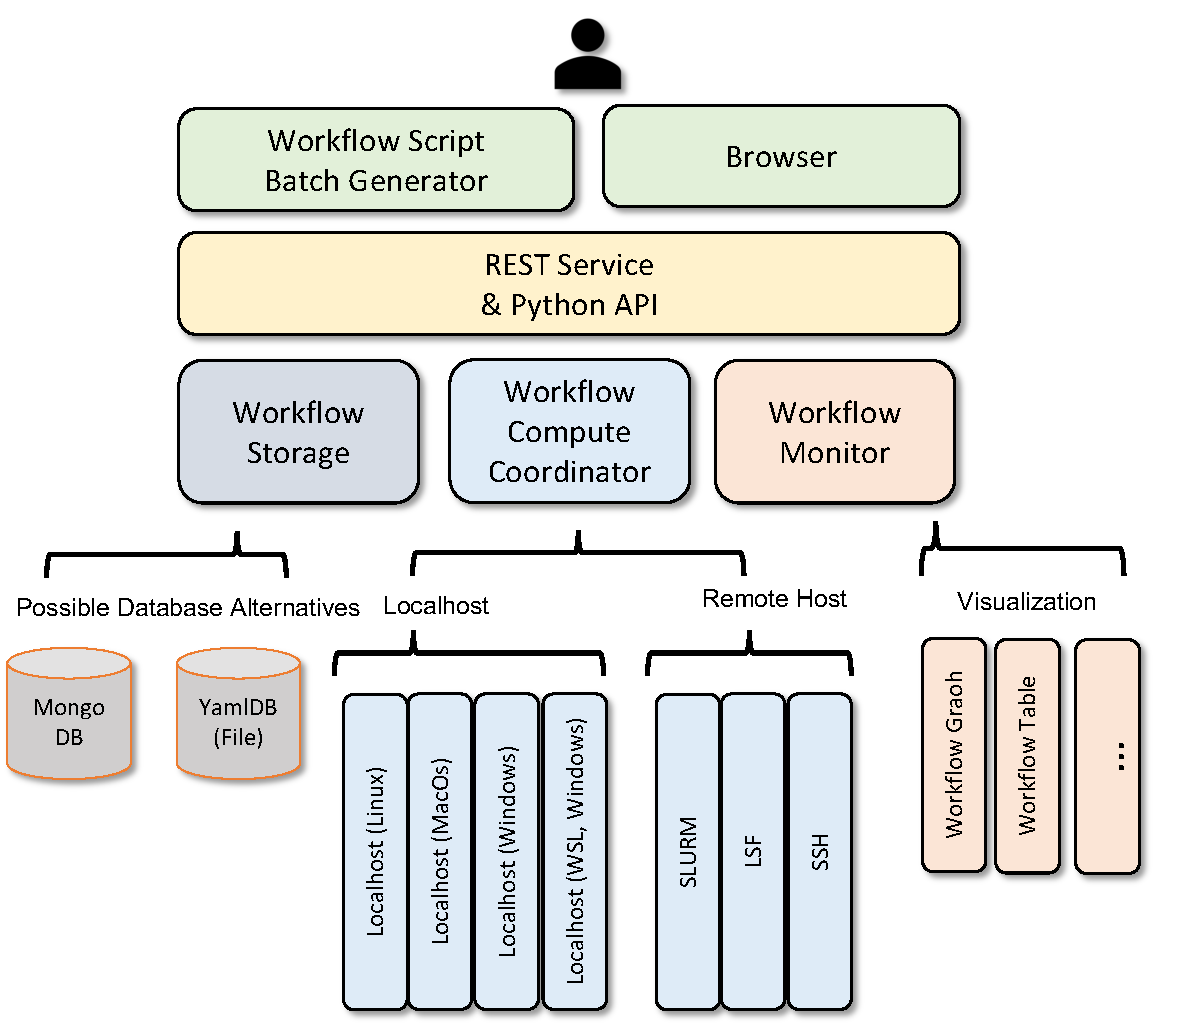
\includegraphics[width=0.50\columnwidth]{images/cloudmesh-cc-new.pdf}
    \caption{Architecture Workflow Service.}
    \label{fig:cc-2}
\end{figure}

Instead of focusing on the details of this architecture, we found that
the high-level use of it is very important as part of the educational
activities which also have an implication in general on the use within
any research activity.

We identified as part of the  analytics service pipelines
three beneficial concepts (see Figure \ref{fig:service-interaction}).

\begin{itemize}
\item {\bf Selection} -- instead of performing all possible benchmarks a
  specific parameter set is selected and only that is run.  
\item {\bf Competition} -- from a number of runs a result is identified that is better than others. This
  may be, for example, the best of n benchmark runs.
\item {\bf Cooperation} -- A number of analytics components is run
  (possibly in parallel) and the final result is a combination of the
  benchmark experiments run in cooperation. This for example could be
  that the job is split across multiple jobs due to resource
  limitations.
\end{itemize}

In the earthquake code, we have observed all three patterns are used
in the benchmark process.

\begin{figure}[htb]
\centering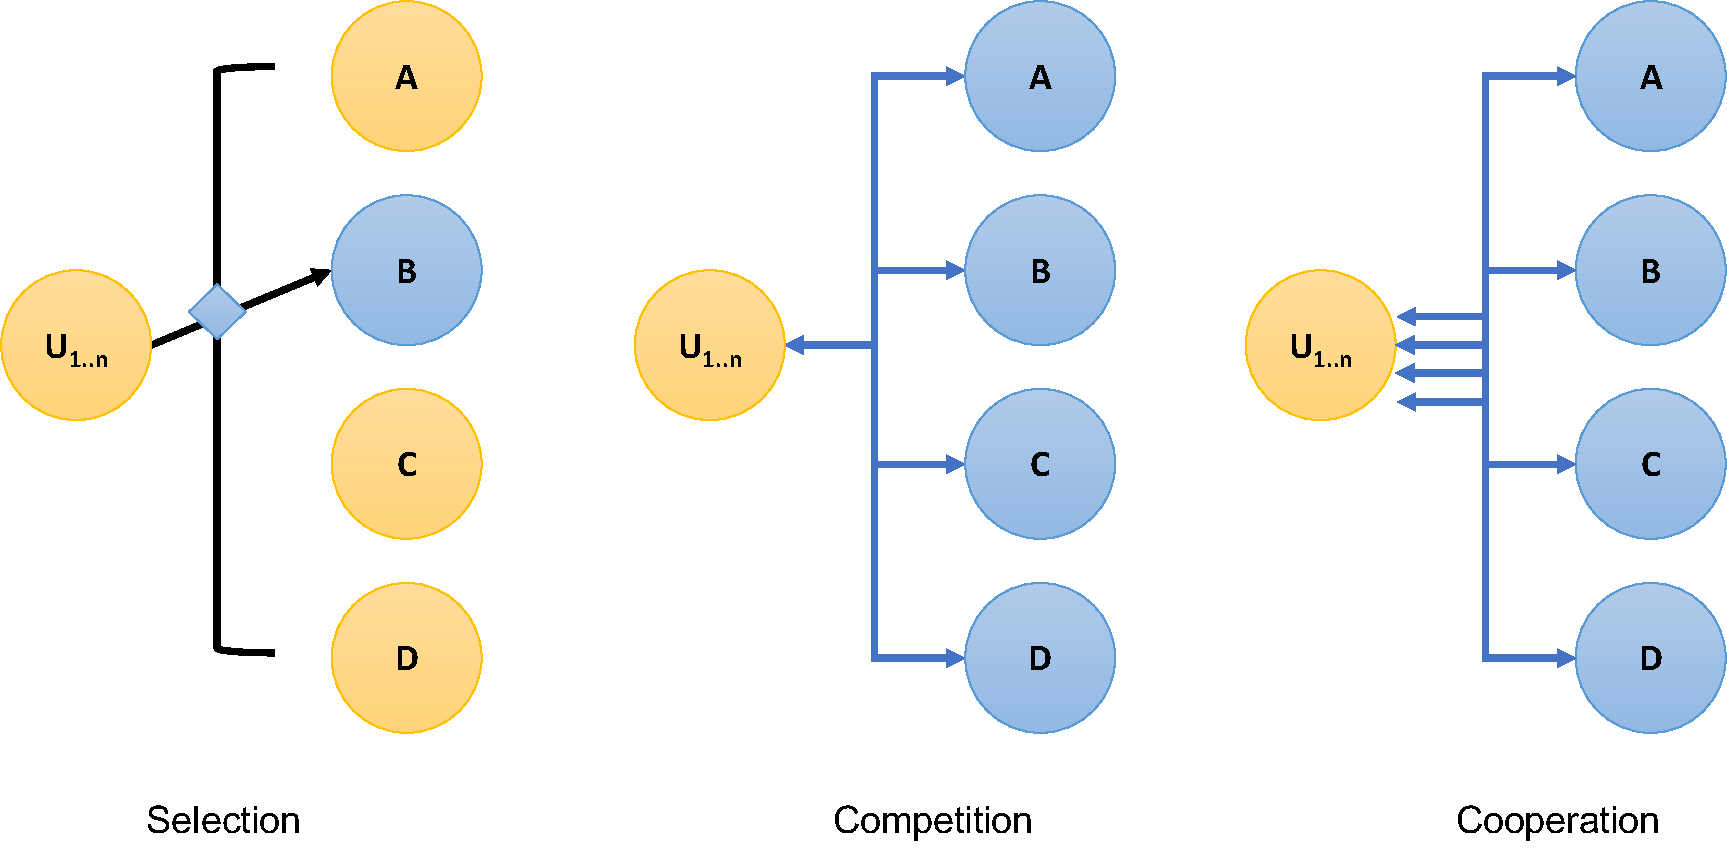
\includegraphics[width=0.75\columnwidth]{images/processes-nist.pdf}
\caption{Service Interaction.}
\label{fig:service-interaction}
\end{figure}




\subsubsection{Workflow Compute Coordinator}
\label{sec:workflow-cc}

% possibly some repitition here

High-performance computing (HPC) is for decades a very important tool
for science. Scientific tasks can be leveraging the processing power
of a supercomputer so they can run at previously unobtainable high
speeds or utilize specialized hardware for acceleration that otherwise
are not available to the user. HPC can be used for analytic programs
that leverage machine learning applied to large data sets to, for
example, predict future values or to model current states. For such
high-complexity projects, there are often multiple complex programs
that may be running repeatedly in either competition or cooperation.
This may include resources in the same or different data centers. We
developed a hybrid multi-cloud analytics service framework that was
created to manage heterogeneous and remote workflows, queues, and
jobs.  It can be used through a Python API, the command line, and a
REST service. It is supported on multiple operating systems like
macOS, Linux, and Windows 10 and 11.  The workflow is specified via an
easy-to-define YAML file.  Specifically, we have developed a library
called Cloudmesh Compute Coordinator (cloudmesh-cc)
\citep{las-22-arxiv-workflow-cc} that adds workflow features to
control the execution of jobs on remote compute resources, while at
the same time leveraging capabilities provided by the local compute
environments to direct interface with graphical visualizations better
suited for the desktop. The goal is to provide numerous workflows that
in cooperation enhance the experience of the analytics tasks. This
includes a REST service (see Figure {fig:fastapi-cc}) and command line
tools to interact with it.


\begin{figure}[htb]
\centering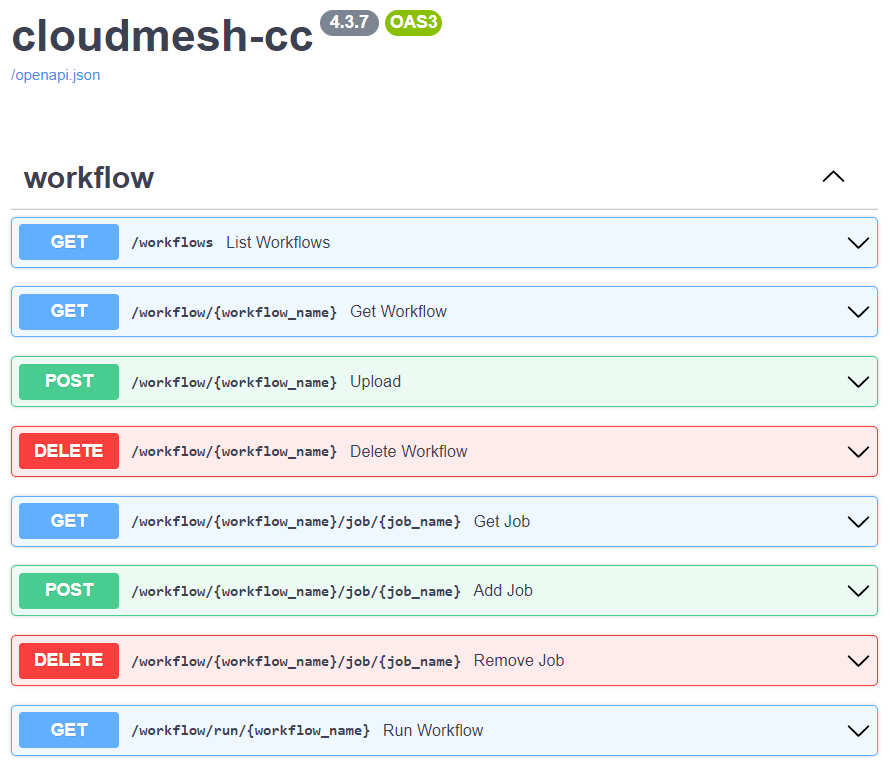
\includegraphics[width=0.7\columnwidth]{images/fastapi-service.png}
\caption{Fast API Workflow Service.}
% better resolution
\label{fig:fastapi-cc}
\end{figure}



\begin{figure}[htb]
    \centering
    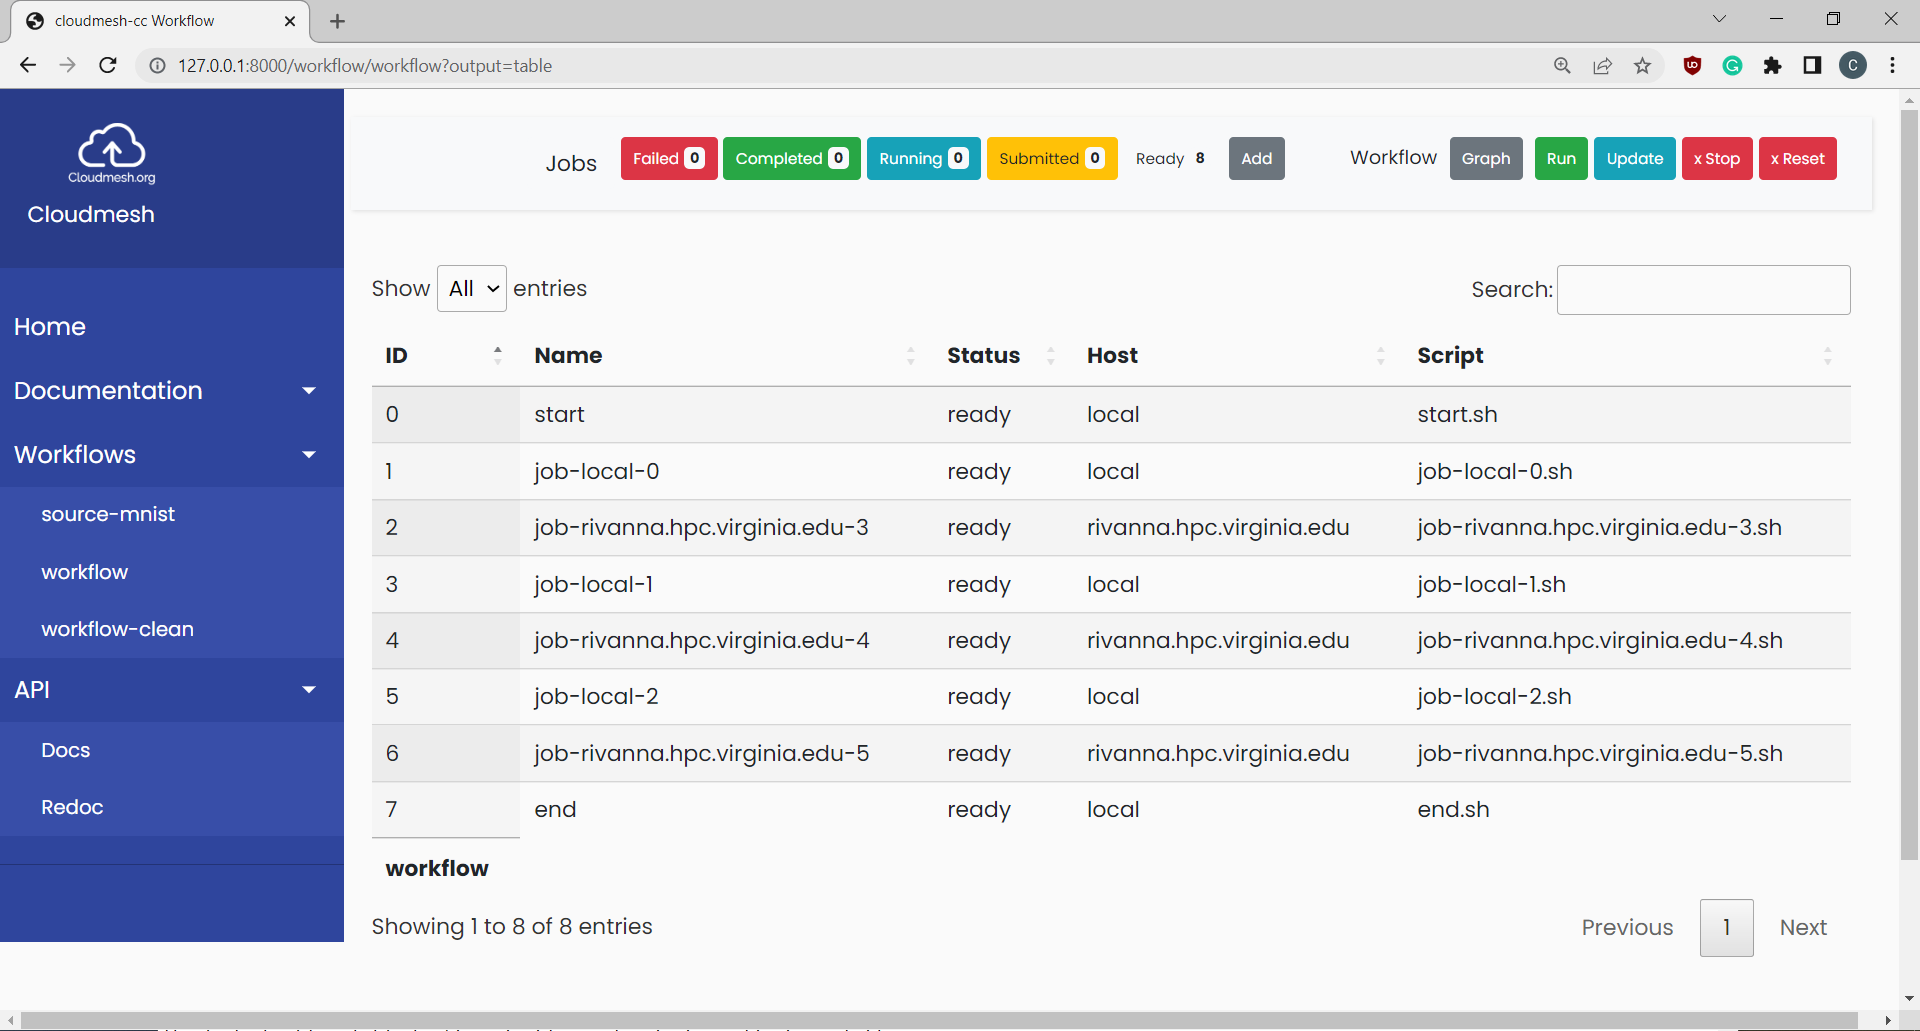
\includegraphics[width=0.70\columnwidth]{images/cc-1.png}
    \caption{Workflow user interface.}
    \label{fig:cc-3}
\end{figure}


We have tested the framework while running various MNIST application
examples, including Multilayer Perceptron, LSTM (Long short-term
memory), Auto-Encoder, Convolutional, and Recurrent Neural Networks,
Distributed Training, and PyTorch training.  A much lager application
using earthquake prediction has also been used.

Figure \ref{fig:fastapi-cc} shows the REST specification and
\ref{fig:cc-2} shows the architecture.

\subsection{Parameterized Workflow Job Generator}
\label{sec:workflow-sbatch}

In traditional machine learning workflows, hyper-parameter tuning and
configuration are key elements in assessing and optimizing the
performance of models. However, scaling hyperparameters for highly
parallel execution with heterogeneous hardware is complex.

Cloudmesh Sbatch is a hyperparameter and configuration management
toolkit designed to address the generation of batch jobs with a
consistent and configurable interface based on hyperparameter values
across multiple development toolchains. One of its functions is to
create batch jobs based on parameterized job specifications and
configuration files.  Cloudmesh-sbatch is part of the Cloudmesh
toolkit, a set of tools and libraries for managing cloud and HPC
resources from the command line, REST interfaces, or GUI's.
Cloudmesh-sbatch can use a variety of
queuing systems and submission commands. Currently, we provide
interfaces to SLURM, LSF, and ssh. As the original system was
developed first for SLURM sbatch submissions we used the name
cloudmesh-sbatch. In the future, we may find a better name showcasing the
generality of the system while using arbitrary queuing systems and
submission commands.

The architecture of the cloudmesh-sbatch framework is depicted in
Figure \ref{fig:cm-sbatch}.

\begin{figure}[htb]
    \centering
    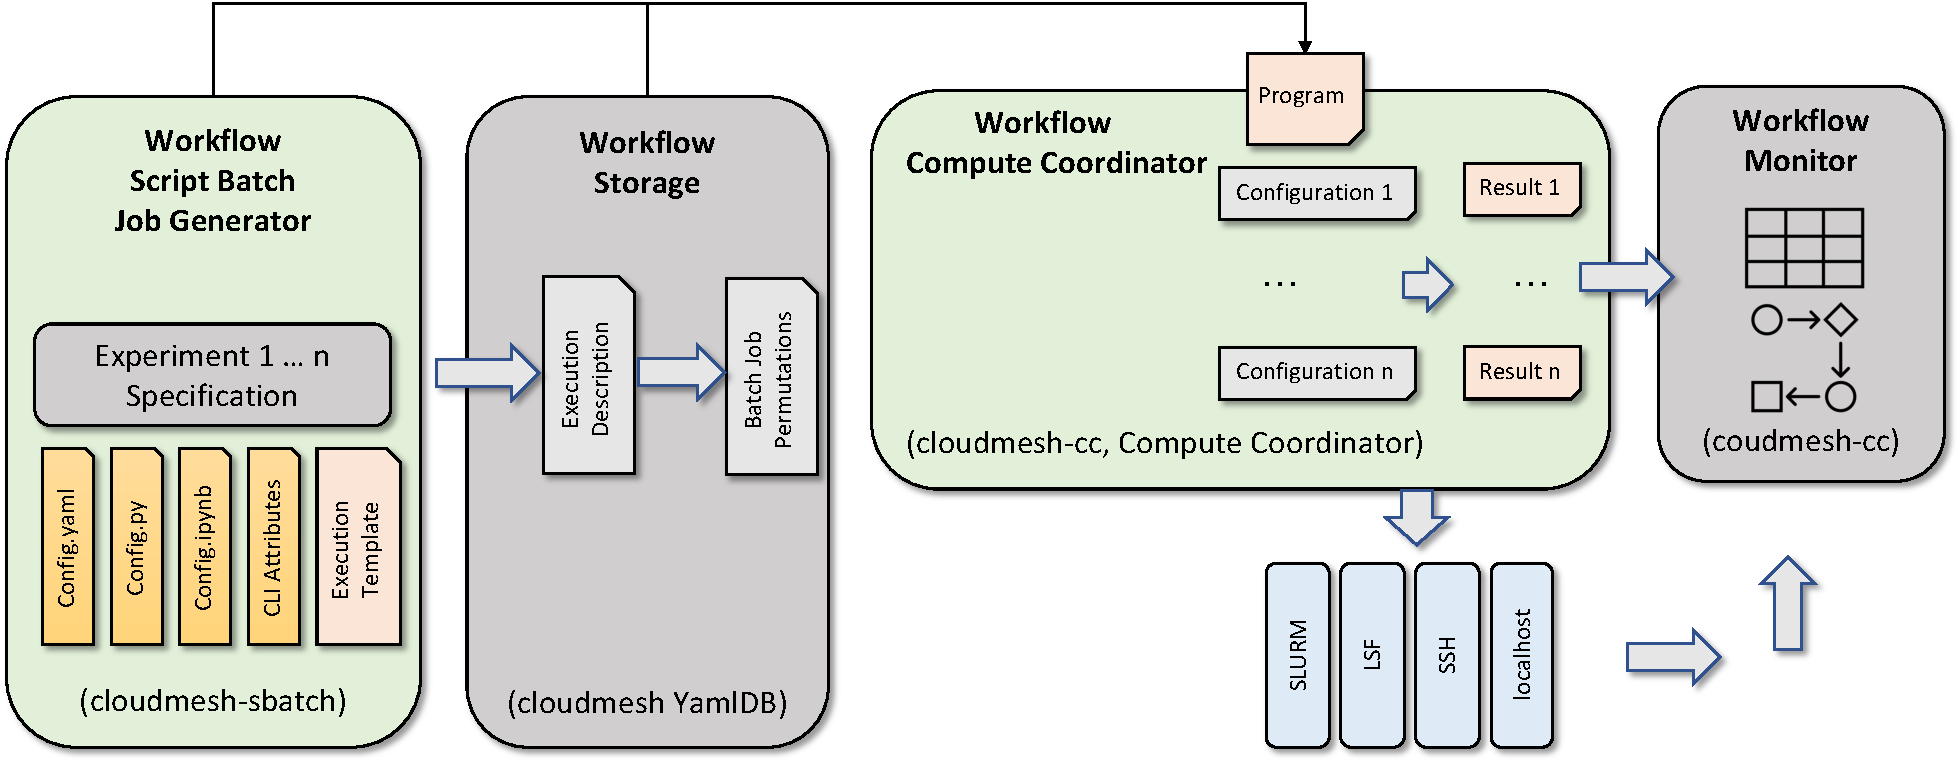
\includegraphics[width=0.70\columnwidth]{images/cloudmesh-sbatch-new.pdf}
    \caption{Workflow Script Batch Generator.}
    \label{fig:cm-sbatch}
\end{figure}


Where cloudmesh-sbatch differentiates itself from other template engines is its
ability to generate a cartesian product  (permutation) of hyperparameter values
underneath of its {\it experiment} heading, making it trivial to
scale an experiment from one execution to thousands of configurations
based on the ranges and their unique combinations.  The resulting
output provides a generated SLURM or LSF script and a YAML
configuration file representing the specific hyperparameters.  By
managing highly configurable jobs with cloudmesh-sbatch, the focus is
placed on what hyperparameters to use for experiments and reduce the
possibility of human error when running experiments over a range of
hyperparameters.

Cloudmesh-sbatch takes two configuration files. The first is a YAML
file that includes all parameters used by the benchmark including an
experiment section that defines the cartesian product. It will 
create SLURM scripts via cloudmesh-sbatch while

\begin{enumerate}
  \item using a unique directory for the experiment
  \item taking a parameter set from the cartesian product
    of the experiment parameters
  \item creating from a batch job template an instantiation of the
    template while replacing all variables from the configuration file
    and replacing the specific experiment parameters
  \item creating an instantiation of the configuration file while replacing all experiment parameters with the one for the current experiment.
\end{enumerate}

This is executed for all permutations of the experiment parameters.

An example of a configuration file \verb|config.yaml| includes

{\footnotesize
\begin{Verbatim}
    application:
        name: earthquake

    data: /scratch/\textcolor{red}{os.USER}/{application.name}
       
    experiment:
        epoch: "1,30,60"
        gpu: "a100,v100"
        repeat: "1,2,3,4,5"
\end{Verbatim}
}

An example of a templated batch script is

{\footnotesize
\begin{Verbatim}
    #!/bin/bash

    #SBATCH --job-name={experiment.repeat}-{application.earthquake}
    #SBATCH --nodes=1
    #SBATCH --gres=gpu:{experiment.gpu}:1
    #SBATCH --time=02:00:00
    #SBATCH --mem=64G
    #SBATCH -o {experiment.gpu}-{application.earthquake}/{experiment.repeat}-%j.out
    #SBATCH -o {experiment.gpu}-{application.earthquake}/{experiment.repeat}-%j.err
    #SBATCH --partition=bii-gpu
    #SBATCH --account=bii_dsc_community

    export USER_SCRATCH=/scratch/$USER
    cd USER_SCRATCH
    mkdir -p $USER_SCRATCH/{experiment.gpu}-{application.earthquake}/%j.out
    nvidia-smi

    cms gpu watch --gpu=0 --delay=0.5 --dense > outputs/gpu0.log &

    python earthquake.py --config config.yaml

    seff $SLURM_JOB_D
\end{Verbatim}
}

The variables can easily be referred to with a dot notation in the
templates.  Variables in the YAML file can also be replaced so it is
possible to use abbreviations easily and in a consistent fashion in
the YAML file as well as in the batch script.

The configuration files and cloudmesh-sbatch can be configured with
parameters so that the files and directories are placed in the right
location and repeatable experiments are created not only on the
original machine but the template can also be easily adapted onto
other machines. An example of a variable replacement specification in
YAML file is given for the \verb|data| value where not only the
operating system variable \verb|os.USER| is replaced, but also the
variable \verb|{application.name}|. Obviously, this is a significant
functionality enhancement to a typical YAML file.  Multiple values are
only possible under the experiment tag, where a variable with multiple
values is assigned a string with multiple values separated by commas.

One can choose a number of important parameters as part of the
permutation strategy to create different experiments. Common variables
are names of graphics cards (if available), memory, file systems used,
versions of Python, versions of TensorFlow, epochs, learning rate, and
many other important parameters that can influence the benchmark.  The
reason why we only allow the parameters with variation under
\verb|experiment| is to assure that there is no confusion with other
parameters that may not be modified and instead only represent a
single value. However, variables under experiment are allowed to have
just a single value.  Another interesting case is the introduction of
a repeat parameter, allowing the program to be executed multiple times
in order to for example support patterns of competition or
collaboration while selecting best values, or creating averages.


The final output of cloudmesh-sbatch is a shell script that contains
all jobs that are to be executed with the defined permutations over the
parameters.

One nice side effect of this is that the jobs in the file can be run
in parallel and have the queuing system take over the scheduling of
the job following the system-defined queuing policies. However, it may
also be possible to create a {\it collaborative group} submission ,
using our earlier introduced collaborative pattern, where multiple
users submit a portion of the jobs so that policies restricting the
number of jobs per user can be avoided. Furthermore if access to
multiple HPC machines is available the jobs could be split among the
different machines. However, the in that case time measurements may
not be a useful parameter. However, as in the science group, we are
concerned about accuracy the combination of a system comprised of
multiple resources is possible and meaningful.

Our progress with the earthquake benchmark would not have been
possible if we would not have cloudmesh-sbatch. One important aspect
is that the management of thousands of jobs that we ran was simplified
and the jobs could be created easily while fostering
reproducibility. The resulting jobs were run over a time period of a
month, while each job took many hours to complete.





\section{Earthquake Forecast Performance Measurements}
\label{sec:perf-main}


\subsection{Measuring Runtime}
\label{sec:perf-runtime}


The code was significantly modified by removing other code that was
not related to the earthquake prediction application. This included
removing code for hydrology, and COVID prediction that used the same
DL prediction algorithm but with different data and optimization
parameters. To be able to obtain the runtime the code was augmented
with the cloudmesh StopWatch methods to report on relevant start,
stop, status, and event actions. In addition, we augmented the
execution of the batch scripts with code that reports energy and
temperature.

\subsection{Perfomance projection}


Through this augmentation it was possible to identify a projected
runtime on various systems while running at predifined
times. Figure~\ref{fig:performance-projection} shows such a predition
for a machine that has RTX3090 GPU. This machine performs quite fast
as it not only has large fast memory (128MB), but also stores all the
data on a fast NVMe. In fact, this machine was faster that the
available systems at University of Virginia due to its superior file
system performance. As the earthquake application uses lots of data
IO, this makes a big difference and has guided us through the approach
we needed to take on the HPC machine including suggestions for
improving data access speeds to the system staff.

To showcase the different runtimes we showcase the results for a 2
epoch case in Table \ref{tab:2-epoch-case}. To our initial surprise we
found that the RTX3090 machine was originally almost 2.67 times better
than the HPC machine with an A100. Faster processor, better memory,
and especially the fast NVMe instead of a slow NSF mounted filesystem
are the reason for this performance. Initially everyone was surprised
about these numbers, but it lead to suggestions on how to improve
performance by for example adding an NVMe storage and access to a
filesystem locally available to the compute node.


\begin{figure}[htb]
    \centering
    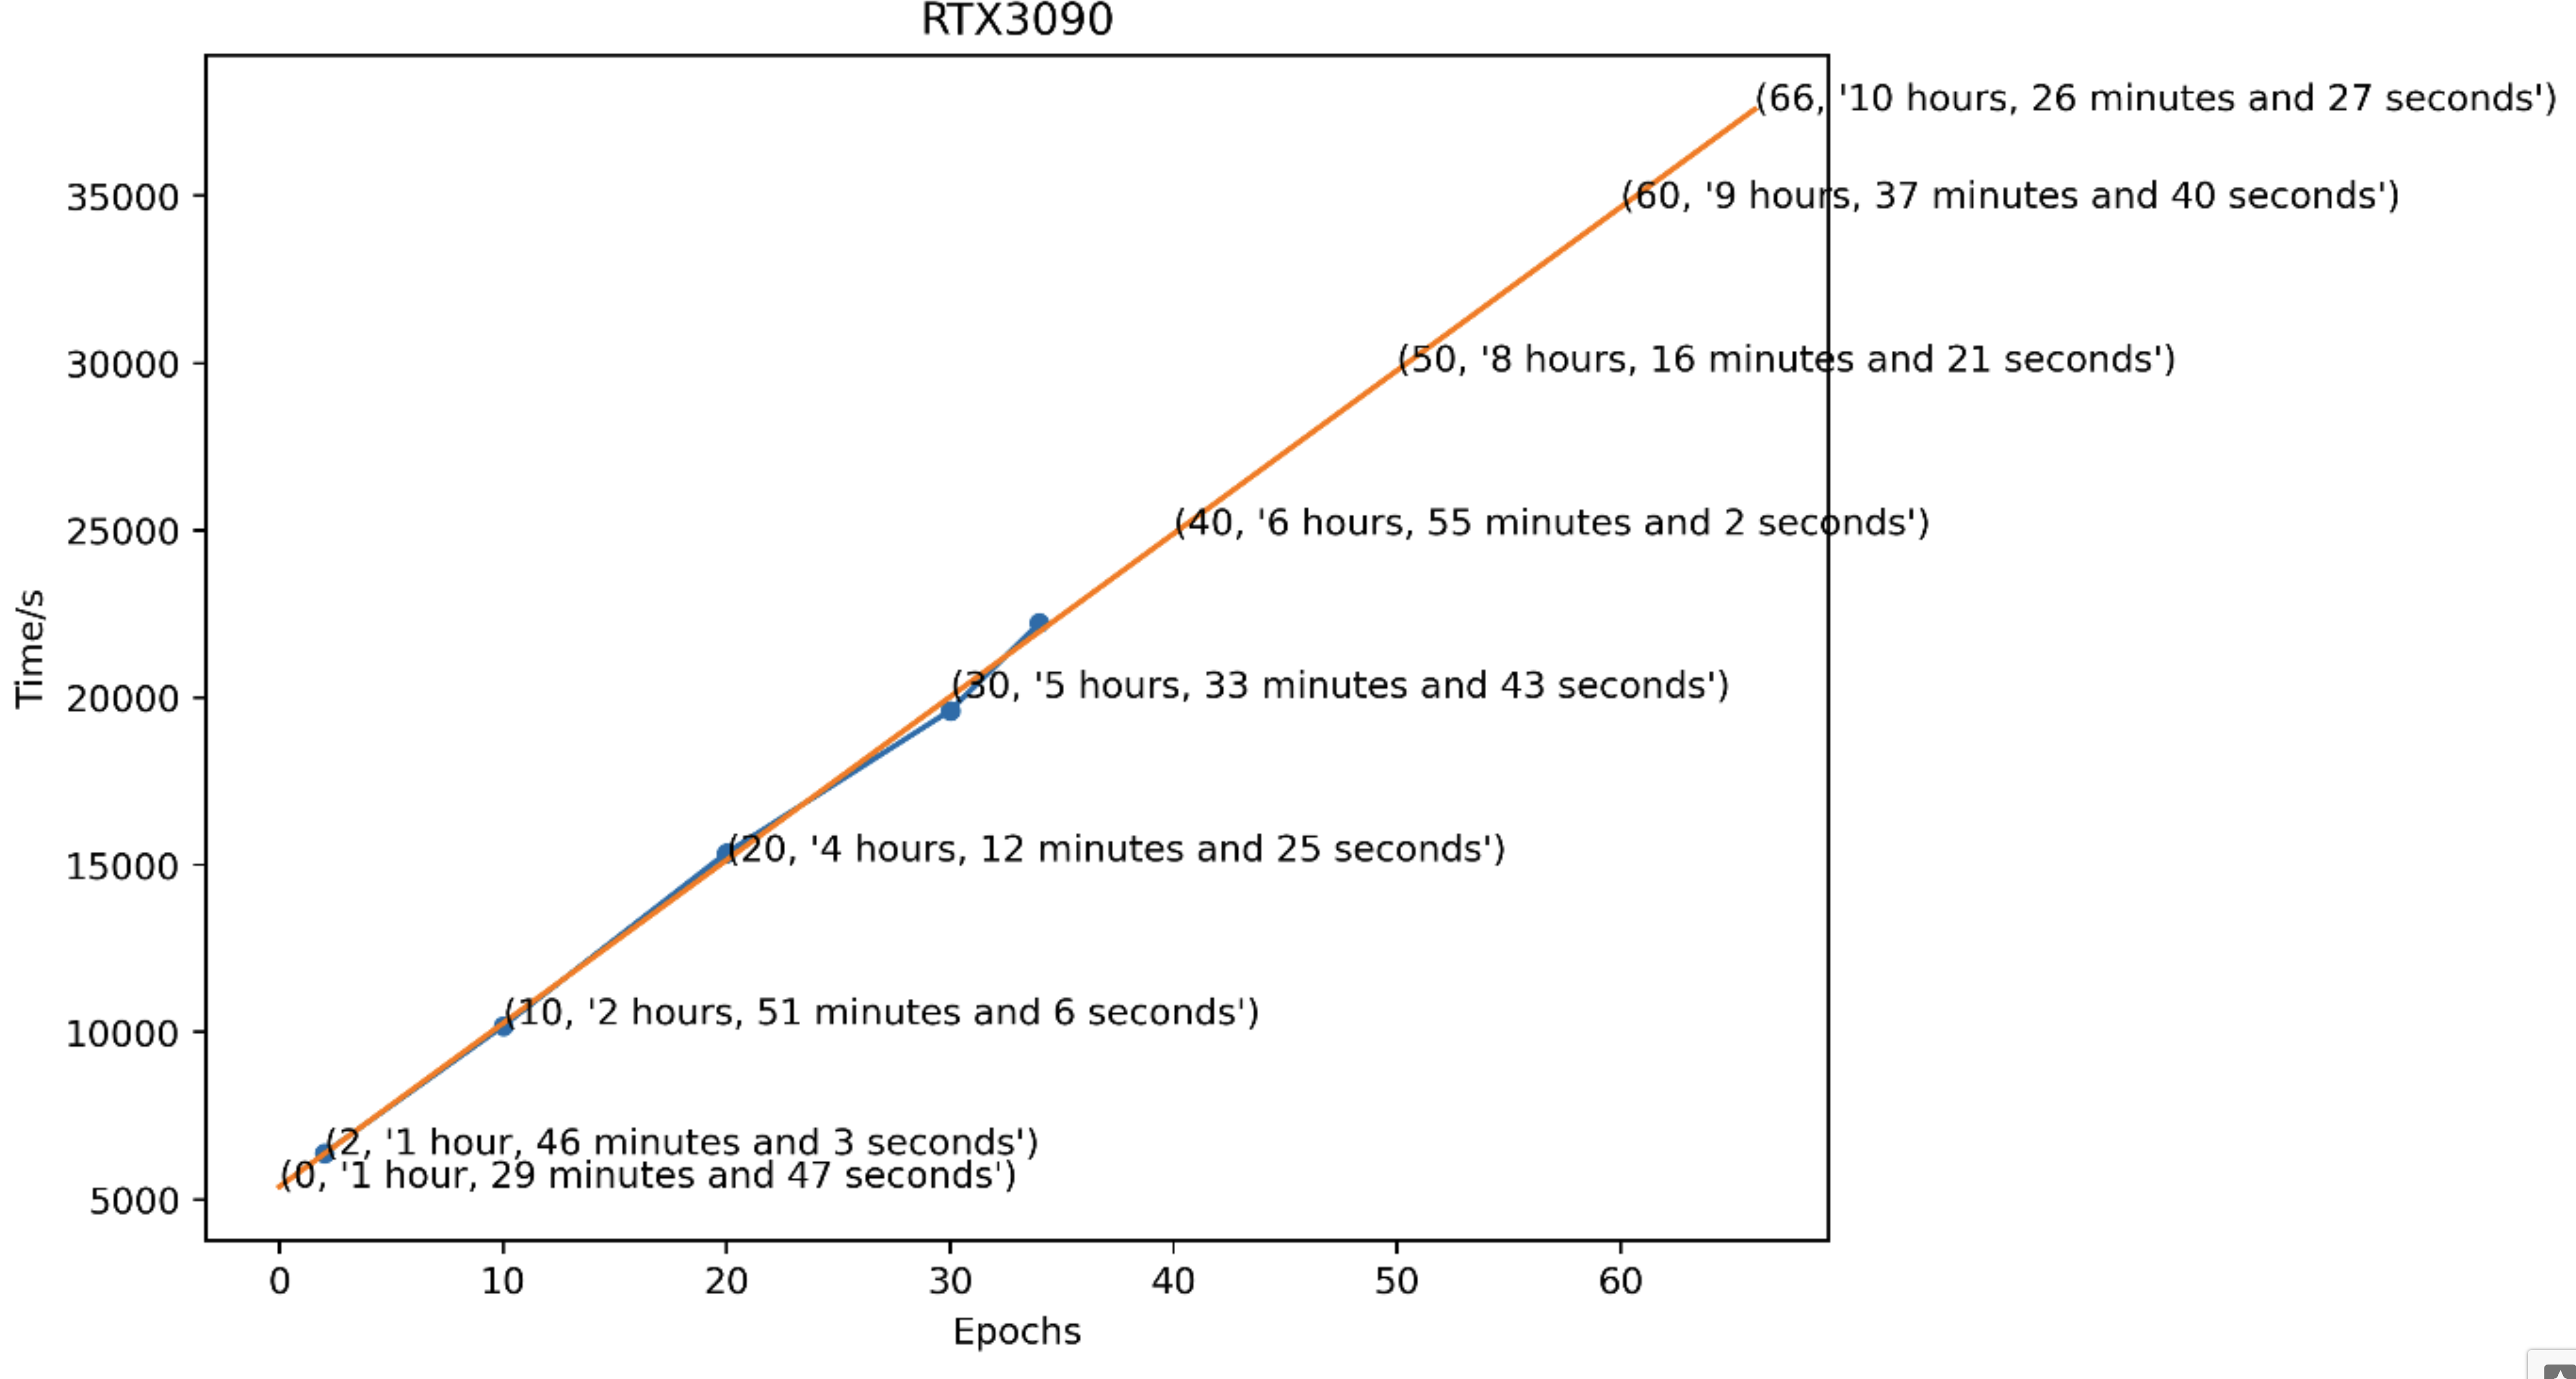
\includegraphics[width=0.70\columnwidth]{images/performance-projection.png}
    \caption{Performance projection. }
    \label{fig:performance-projection}
\end{figure}


\begin{table}[htb]
    \caption{Runtime of the 2 epoch case in seconds}
    \label{tab:2-epoch-case}
    \begin{center}
    {\footnotesize              

          \begin{tabular}{lrrrrr}
            Timer             & RTX3090 & RTX3080 & A100    & V100    & K80     \\
            \hline
            Machine           & Desktop & Laptop  & Rivanna & Rivanna & Rivanna \\
            Total             & 6589.4  & 8348.5  & 17574.8 & 20295.0 & 28343.3 \\
            Sampling location &  457.9  &  532.5  &  1227.0 &  1546.4 &  1779.6 \\
            Init              &    0.8  &    3.6  &    8.1  &     5.6 &     5.3 \\
            Train             & 1103.2  & 2068.9  &  1373.0 &  1671.4 &  6967.3 \\
            Bestfit           & 4420.3  & 4997.1  & 13022.1 & 14795.1 & 17037.6 \\
            \hline
          \end{tabular}

    }
    \end{center}
\end{table}


\subsection{Accuracy Performance Benchmark}
\label{sec:perf-accuracy}

%%% max 15 figures abd table, subfig is one figure

%%%  NB logo1.eps is required in the path in order to correctly compile front page header %%%

As the focus of the MLCommons science working group is the improvement
of the accuracy of an application, we focus our next discussion on
reporting the accuracy of the earthquake application.

We observe that the loss of the application intersects validation and
training at about the epoch value of 30-33 (see Figure~\ref{fig:loss}).  However, we have
constantly also run higher numbers of epochs just to be sure.

\begin{figure}[htb]
    \centering
    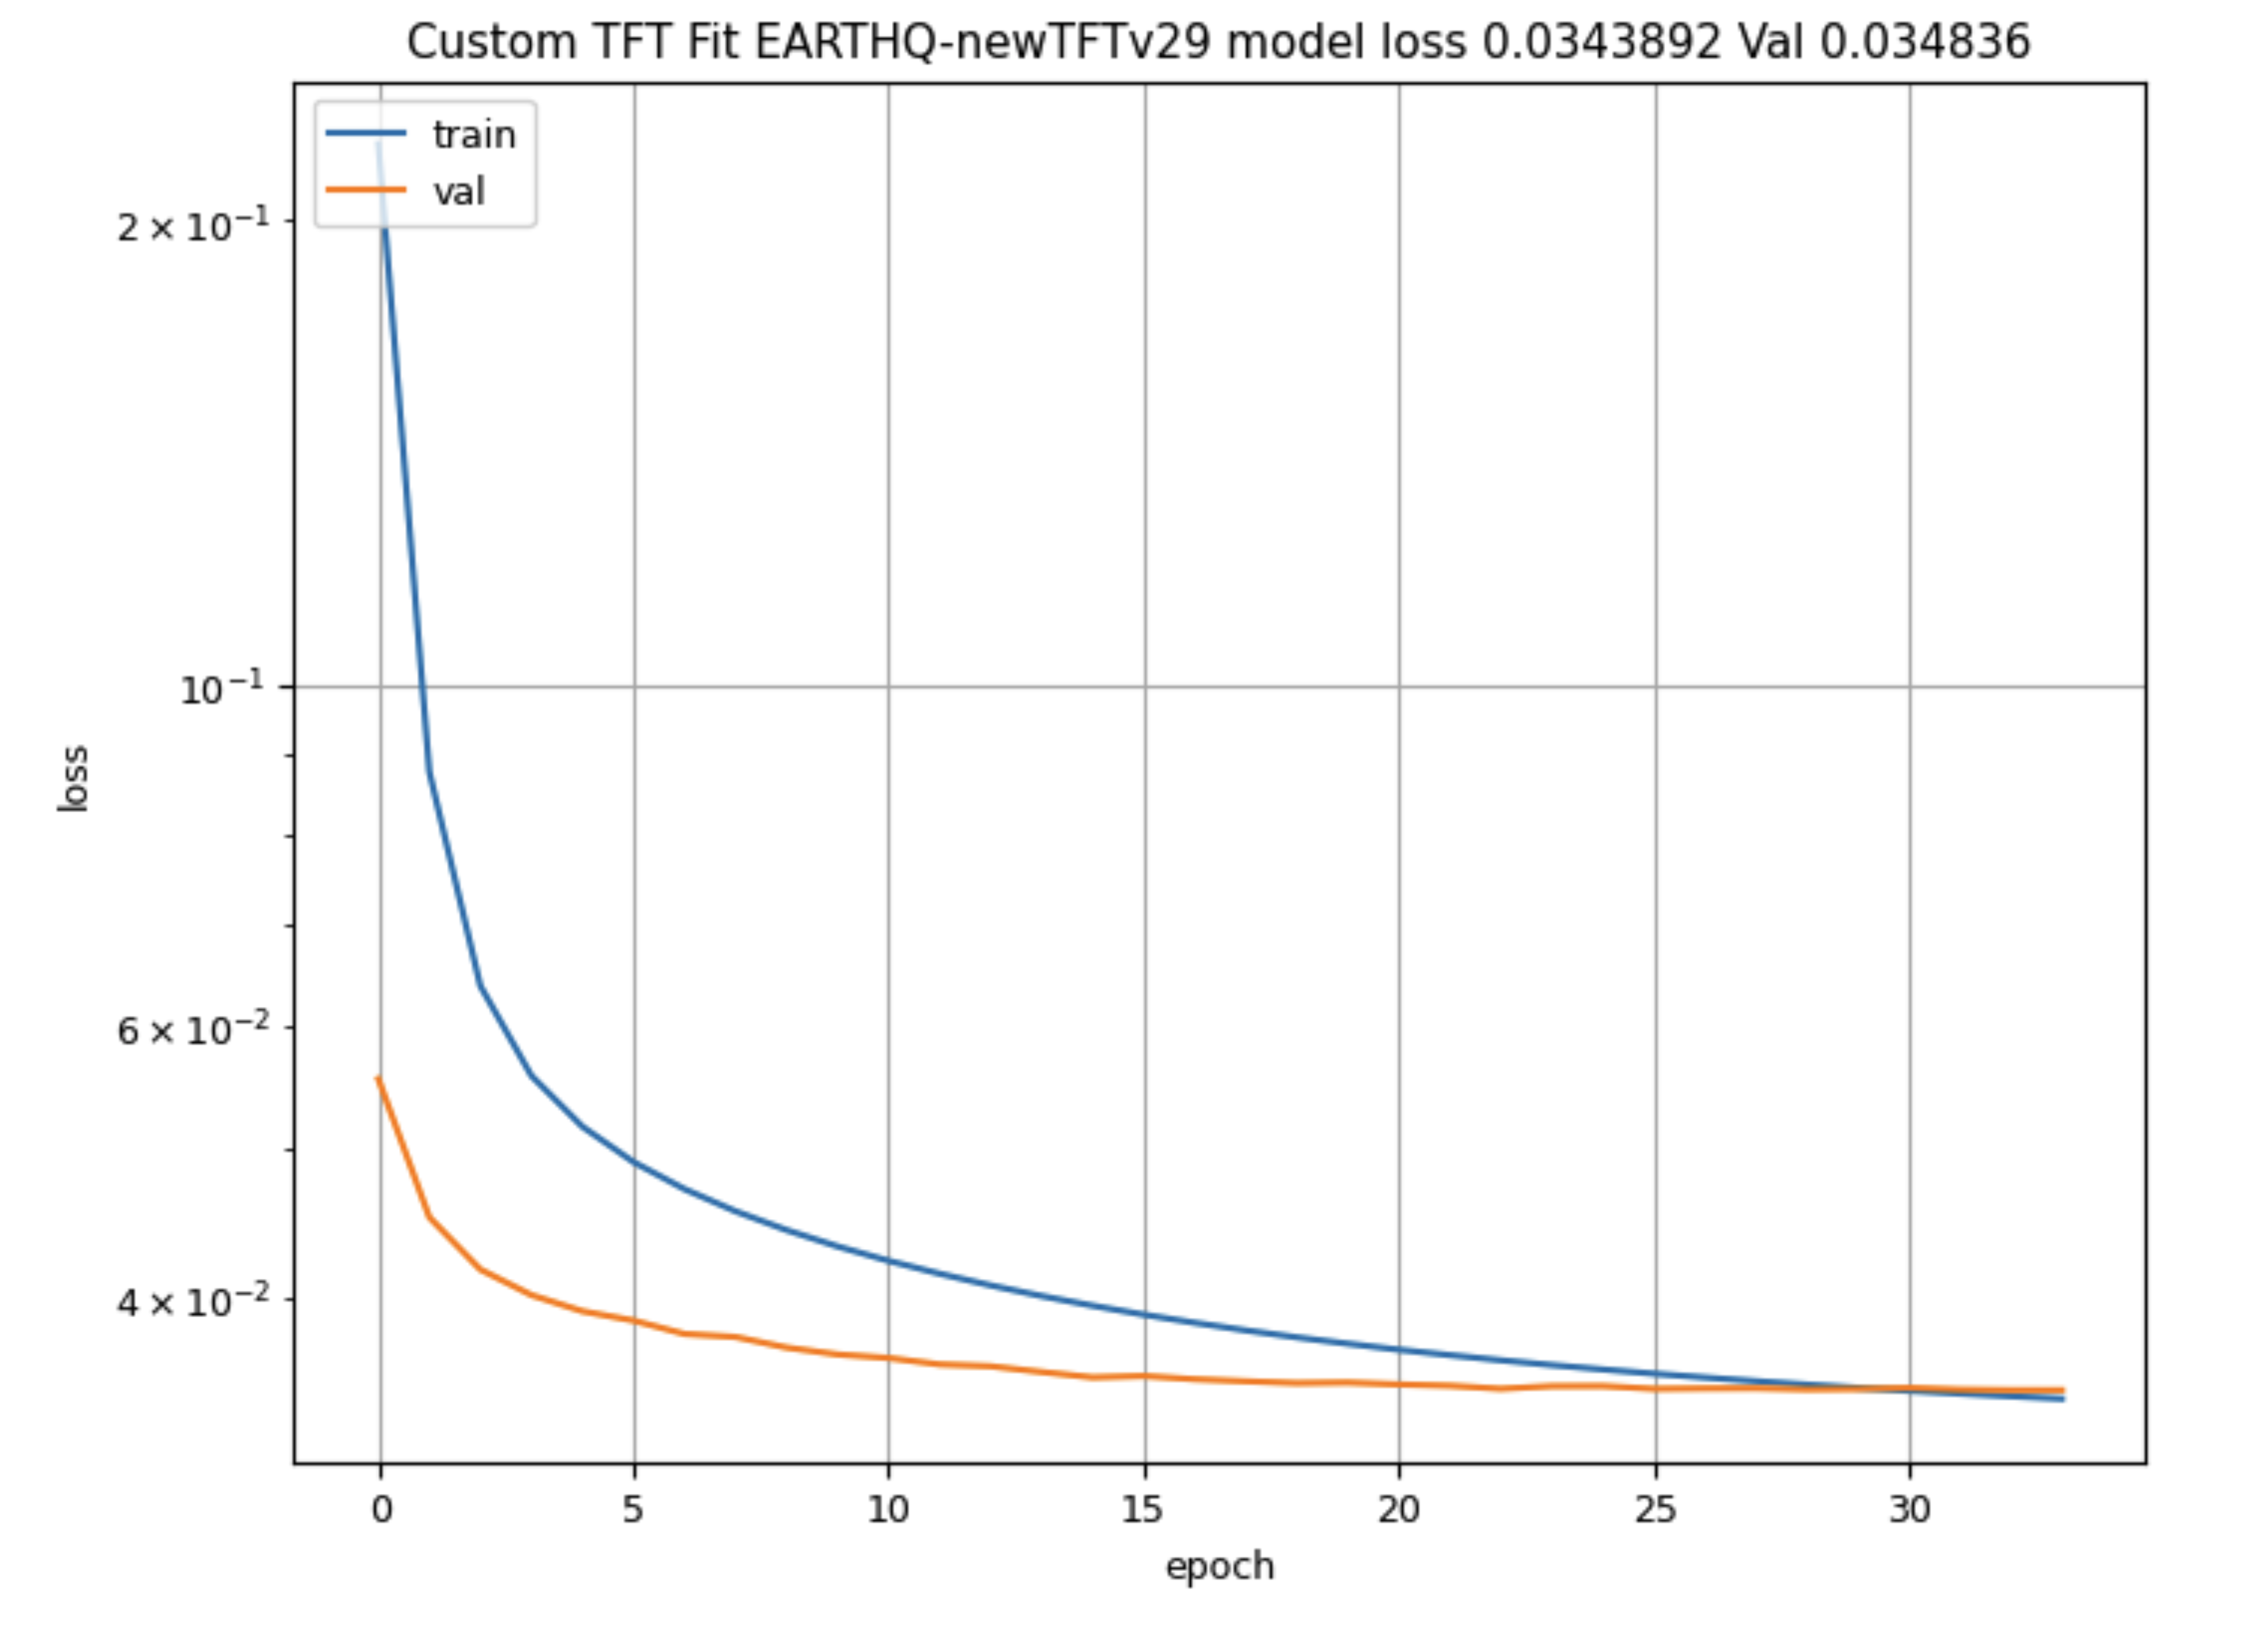
\includegraphics[width=0.70\columnwidth]{images/loss.png}
    \caption{Loss}
    \label{fig:loss}
\end{figure}

Figures~\ref{fig:six-graphs} show accuracy values of NNSE with
various epoch values for training and validation. We chose here 2, 30,
and 70 epochs.  We have then created tables for the NNSE values for
each of the epochs and sorted them by value. The higher the NNSE
accuracy value is the better. We have created tables for the 2, 30,
and 70 epoch hyper-parameters. In addition, we highlighted in the table
the best training value with red, the second best with blue, and the
third best with three. We also highlighted the corresponding value in
the inference column that corresponds to the hyperparameter for the
time period used in the input and output parameters. While we see for
the 2 and 30 epoch cases the same order for these three values, we see
a different order for the 70 epoch case. This can be explained through
overfitting. Overall we find that the best accuracy can be found for

An epoch value of 30  and the hyperparameter {\em Now 2wk+26AV} which has an NNSE value for the training of 
0.5218 and a validation value of 0.502300 


\TODO{To be simplified by Thomas}

In the following benchmarks a number of hyper parameters were used to
determine the training data that derive accuracy values with the
earthquake benchmark code.

All time data is grouped into 2 week time periods.

We distinguish the following abbreviations. The first term defines the
start point for the first training time period before the current date
the model is on. In the case of Now the start point is the current
date.

The second parameter has two values 2wk+xAVG where x is a number. The
first defines a 2 week time period denoted by 2wk. The second defines
how many total time groups are put in the training data.

In addition we also have the values which only have one time period, 3
Months Back, 6 Months Back, Year Back and 2 weeks Now.

Some examples are:
\begin{itemize}
\item {\bf Now 2wk+26AVG} -- 2 week training time periods at the
  current date and ending after 26 total time periods are reached.
\item {\bf 3M 2wk+13AVG} -- 2 week training time periods starting at 3
  months before the current date and ending after 13 total time
  periods are reached.
\item {\bf 1Y 2wk+7AVG} -- 2 week training time periods starting at 1
  year before the current date and ending after 7 total time periods
  are reached.
\item {\bf 6 Months Back} -- 2 week training time periods starting at
  6 months before the current date and ending after 1 time period is
  reached.
\item {\bf Year Back} -- 2 week training time periods starting at 1
  year before the current date and ending after 1 time period is
  reached.
\item {\bf 3 Months Back} -- 2 week training time periods starting at
  3 months before the current date and ending after 1 time period is
  reached.
\item {\bf 2 weeks Now} -- 2 week training time periods starting at
  the current date and ending after 1 time period is reached.
\end{itemize}



\begin{table}[htb]
  \caption{The top 20 accuracy values based on hyperparameters with 2,
    30, and 70 epochs}
  \label{tab:ranking-accuracy}
  \renewcommand{\arraystretch}{1.2}
  \begin{center}
    {\footnotesize  
\begin{tabular}{|l||r|r|l|r|r|l|}
  \hline
 &   \multicolumn{3}{c|}{\bf \textcolor{red}{Training}}  & \multicolumn{3}{c|}{\bf \textcolor{blue}{Validation}}  \\
{\bf Rank} &  {\bf NNSE} &  {\bf Epoch} & {\bf Hyper-parameter} & {\bf NNSE} &  {\bf Epoch} & {\bf Hyper-parameter}\\
\hline
\textcolor{red}{1}  &  \textcolor{red}{0.6930} &     \textcolor{red}{70} &  \textcolor{red}{Now 2wk+26AVG} &  \textcolor{blue}{0.5582} &     \textcolor{blue}{70} &  \textcolor{blue}{Now 2wk+26AVG} \\
2  &  0.6681 &     70 &  Now 2wk+26AVG &  0.5487 &     70 &  Now 2wk+26AVG \\
3  &  0.6549 &     70 &  Now 2wk+13AVG &  0.5377 &      2 &    2 weeks Now \\
4  &  0.6419 &     30 &  Now 2wk+26AVG &  0.5292 &      2 &  Now 2wk+26AVG \\
5  &  0.6371 &     30 &  Now 2wk+26AVG &  0.5246 &     30 &  Now 2wk+26AVG \\
6  &  0.6295 &     70 &  Now 2wk+13AVG &  0.5156 &     70 &  Now 2wk+13AVG \\
7  &  0.6274 &     70 &   Now 2wk+7AVG &  0.5150 &     30 &  Now 2wk+26AVG \\
8  &  0.6178 &     30 &  Now 2wk+26AVG &  0.5133 &     30 &  Now 2wk+26AVG \\
9  &  0.6101 &     30 &  Now 2wk+26AVG &  0.5050 &     70 &  Now 2wk+13AVG \\
10 &  0.6063 &     30 &  Now 2wk+13AVG &  0.5034 &     30 &  Now 2wk+26AVG \\
11 &  0.6009 &     70 &   Now 2wk+7AVG &  0.4975 &     30 &  Now 2wk+26AVG \\
12 &  0.5978 &     30 &  Now 2wk+13AVG &  0.4897 &     70 &   Now 2wk+7AVG \\
13 &  0.5948 &     70 &    2 weeks Now &  0.4860 &     30 &  Now 2wk+13AVG \\
14 &  0.5900 &     30 &  Now 2wk+26AVG &  0.4766 &     70 &   Now 2wk+7AVG \\
15 &  0.5880 &     30 &   Now 2wk+7AVG &  0.4766 &     30 &  Now 2wk+13AVG \\
16 &  0.5864 &     30 &  Now 2wk+13AVG &  0.4734 &      2 &  Now 2wk+13AVG \\
17 &  0.5818 &      2 &    2 weeks Now &  0.4675 &     70 &  Now 2wk+26AVG \\
18 &  0.5790 &     30 &   Now 2wk+7AVG &  0.4631 &     30 &   Now 2wk+7AVG \\
19 &  0.5786 &     30 &    2 weeks Now &  0.4618 &     30 &    2 weeks Now \\
20 &  0.5696 &     70 &    2 weeks Now &  0.4594 &      2 &  Now 2wk+26AVG \\
\hline
\end{tabular}
}
\end{center}
\end{table}


%we have finalized the EQ code but want to make absolutely sure that we
%look at the correct values for the scientific comparison.
%
%This also requires a small sentence to each variable. Could we have a
%small meeting and I take then some notes on what these values are
%tomorrow. I will then add the explanations to the MLCommons EQ benchmark
%policy document.
%
%I just want to make sure I understand over which domain we average and
%sum up.
%
%Also if we were to just do one value (just in case they ask, I think we
%would use the summed up total right. However I think it is better to
%keep all of them.)
%
%Also I forgot what the +26 refers to
%
%I think something like this is almost correct, but we need to +26
%explanation and get verification from you.
%
%The Magnification based on a years worth of back data, while looking two
%weeks ahead + 26 what?



code management is important, github is essential
Need to have better sbatch to make code management easier
cluster design is important and access to local storage on nodes is important
shared file systems are less effective 
Predicting behavior of code is great with our timer library as it allows us to estimate runtines and report results in easy fashion. Helps debugging.
Need to look into the implementation of bestfit 
Need to look into memory dependency of epochs
Should we stop at 34 epochs or run 66?

\TODO{add k80 elsewhere}




\subsection{Energy}
\label{sec:perf-energy}


While observing initially the fat runtime of the RTX3090 on a custom
desktop in contrast to the A100 performance on the HPC we were asked
to provide evidence that we use the A100 processor. The energy monitor
we developed and intermittent event notifications throughout the
program provided evidence that we used the machine properly. The
energy traces are generated periodically every second. The traces for
2, 30, and 70 epochs are depicted in Figure \ref{fig:energy-graphs}.


\citep{green500}


\begin{figure}[htb]

  \begin{center}

     \begin{minipage}[b]{0.40\textwidth}
       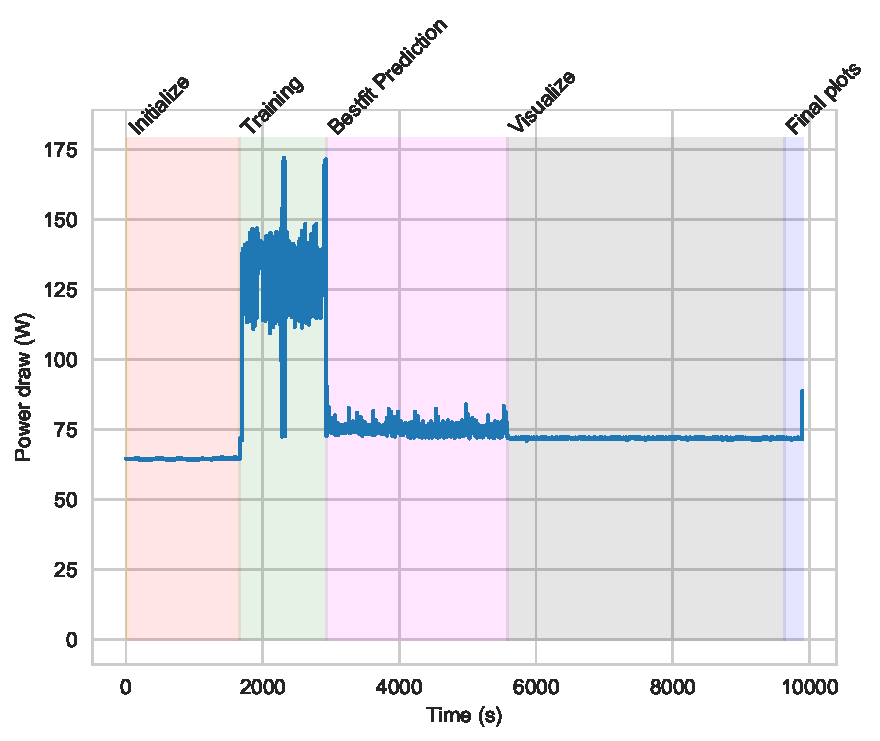
\includegraphics[width=1.0\linewidth]{images/a100-shaded-energy-2-epochs.pdf}
        {\bf (A)} A100 Energy trace for 2 epochs training and validation.
    \end{minipage}
     \ \
     \begin{minipage}[b]{0.40\textwidth}
        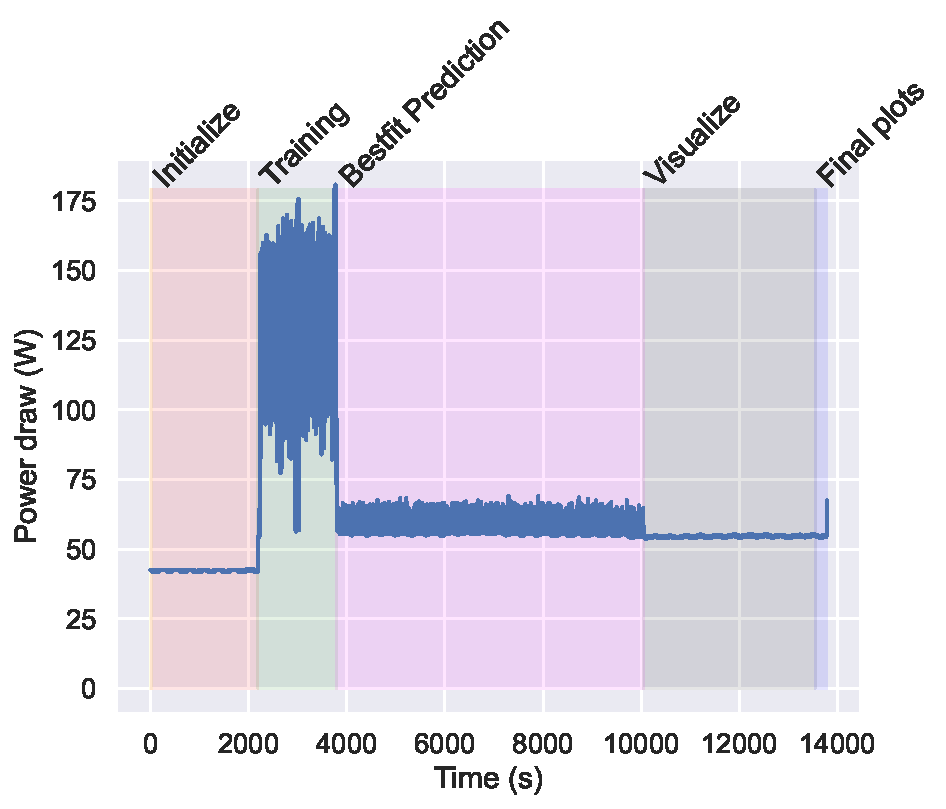
\includegraphics[width=1.0\linewidth]{images/v100-shaded-energy-2-epochs.pdf}
        {\bf (B)}  V100 Energy trace for 2 epochs training and validation.
     \end{minipage}

     \begin{minipage}[b]{0.40\textwidth}
        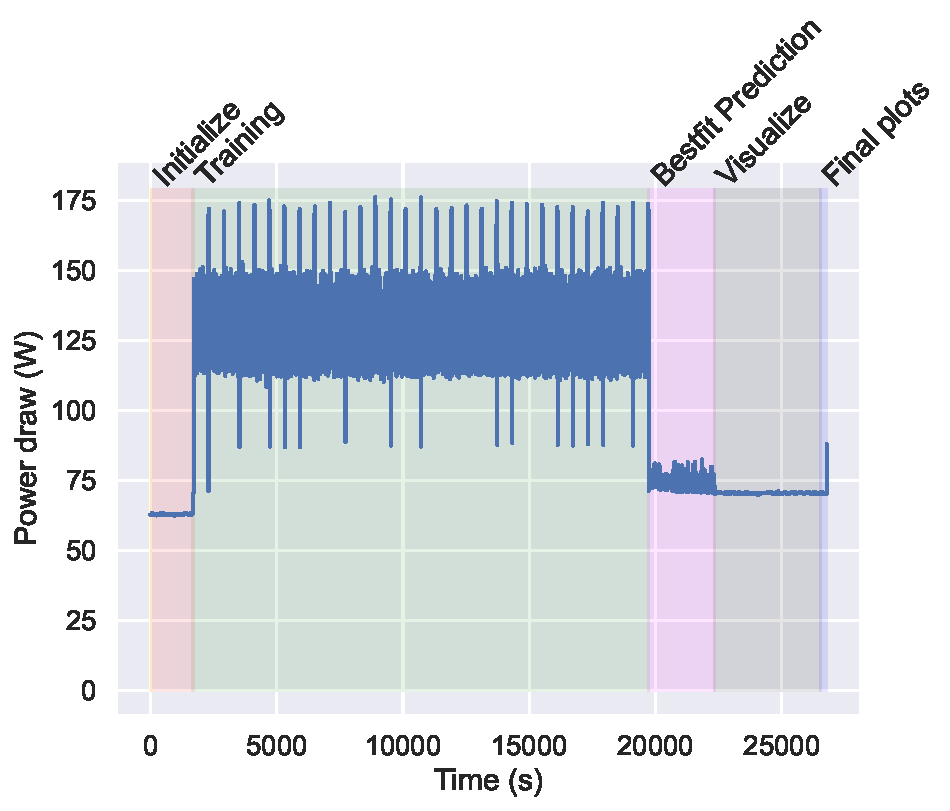
\includegraphics[width=1.0\linewidth]{images/a100-shaded-energy-30-epochs.pdf}
        {\bf (C)} A100 Energy trace for 30 epochs training and validation.
     \end{minipage}
     \ \
     \begin{minipage}[b]{0.40\textwidth}
        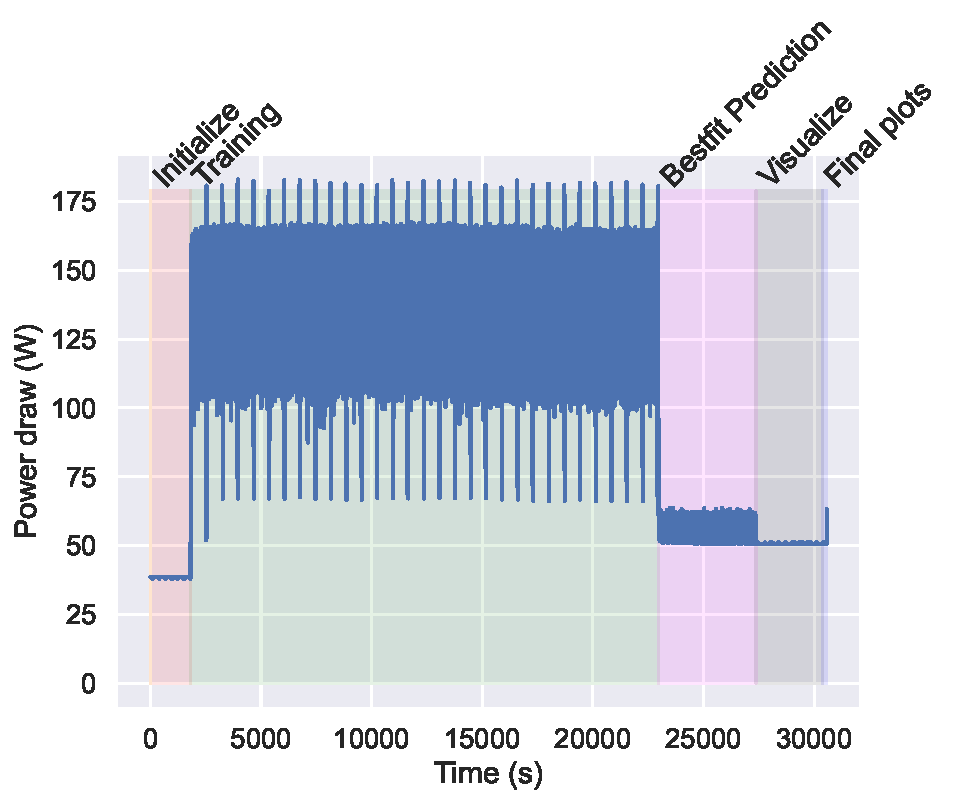
\includegraphics[width=1.0\linewidth]{images/v100-shaded-energy-30-epochs.pdf}
        {\bf (D)} V100 Energy trace for 30 epochs training and validation.
     \end{minipage}

     \begin{minipage}[b]{0.40\textwidth}
       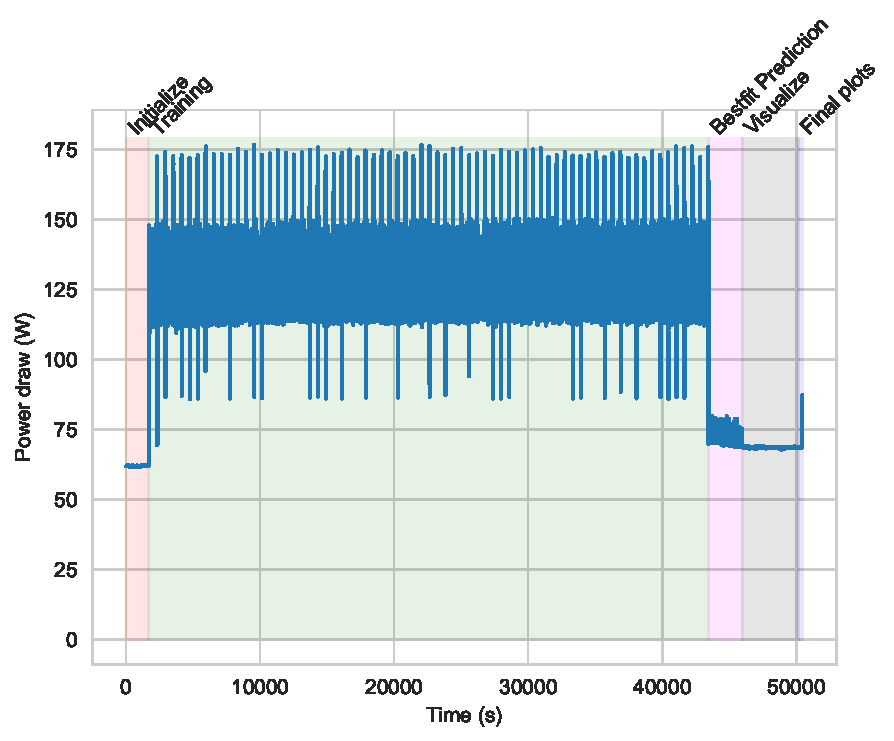
\includegraphics[width=1.0\linewidth]{images/a100-shaded-energy-70-epochs.pdf}
        {\bf (E)} A100 Energy trace for 70 epochs training and validation.
     \end{minipage}
     \ \
     \begin{minipage}[b]{0.40\textwidth}
        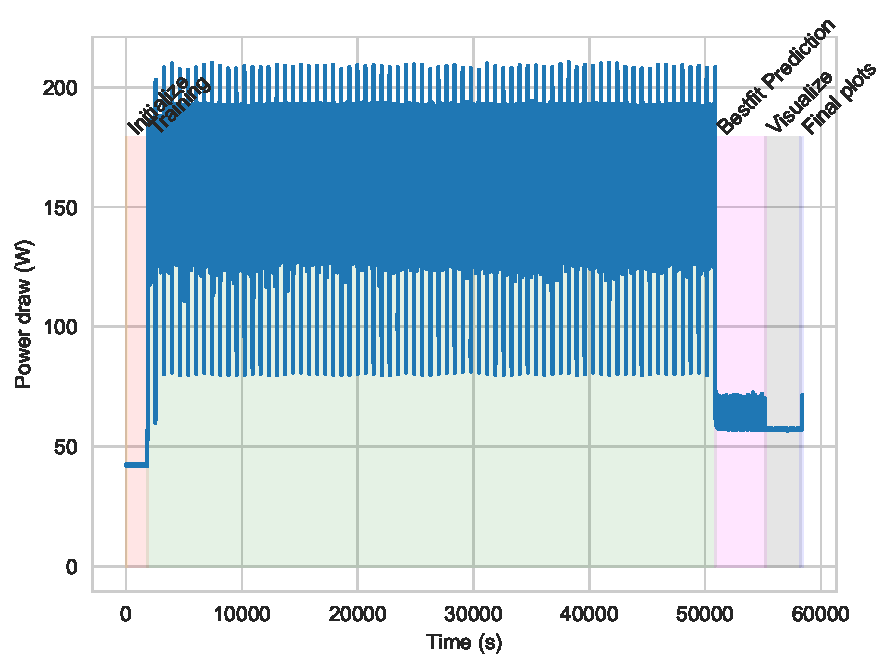
\includegraphics[width=1.0\linewidth]{images/v100-shaded-energy-70-epochs.pdf}
        {\bf (F)}  V100 Energy trace for 70 epochs training and validation.
     \end{minipage}
\end{center}

     \caption{Energy traces for training and validation for epochs 2 (A, B), 30 (C, D), 70 (E, F).}
     \label{fig:energy-graphs}
\end{figure}




\begin{figure}[p]

  \begin{center}
     \begin{minipage}[t]{0.65\textwidth}
        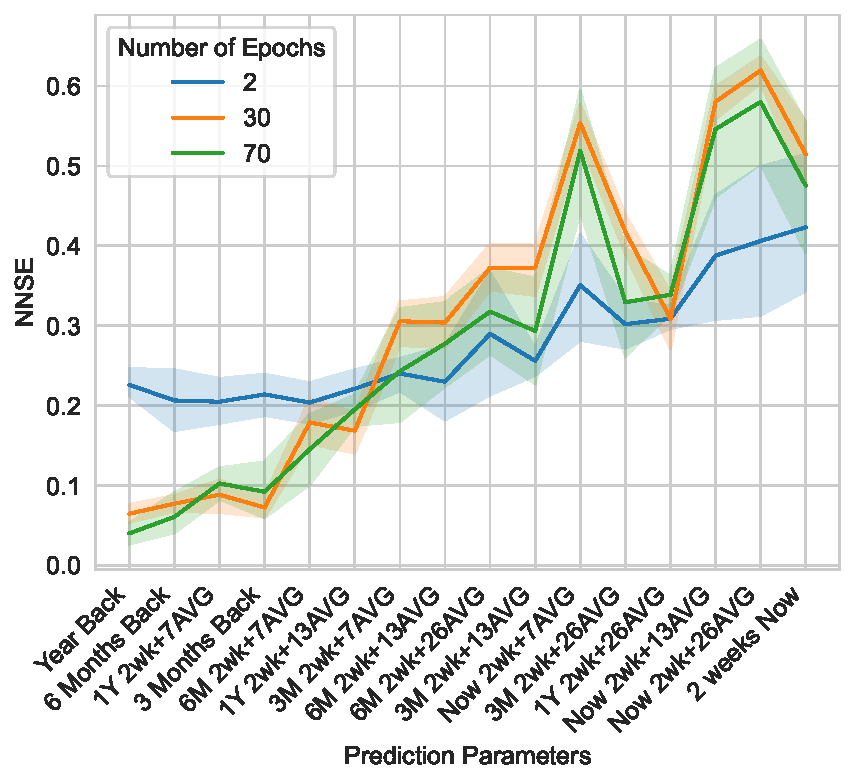
\includegraphics[width=1.0\linewidth]{images/A100-NNSE-all-epochs-training.pdf}
        {\bf (A)} NNSE for training.
     \end{minipage}
  \end{center}
  \ \
  \begin{center}
     \begin{minipage}[t]{0.65\textwidth}
        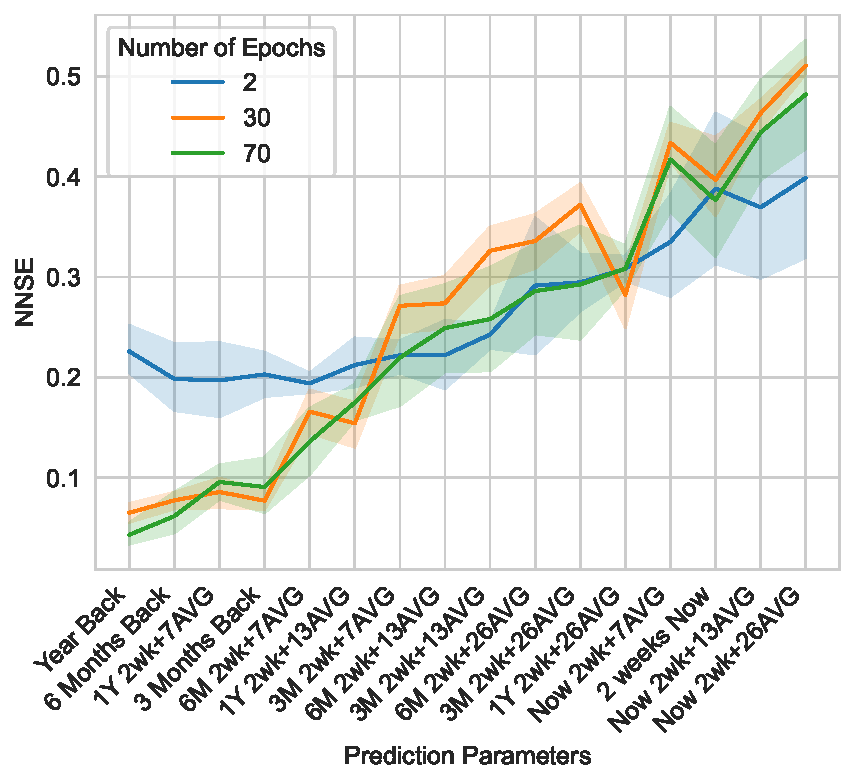
\includegraphics[width=1.0\linewidth]{images/A100-NNSE-all-epochs-validation.pdf}
        {\bf (B)} NNSE for validation.
     \end{minipage}
  \end{center}

  \caption {NNSE comparison}
  \label{fig:NNSE-comparison-a100}

\end{figure}








%%%%%%%%%%%%%%%%%%%%%%%%%%%%%

\begin{comment}
\TODO{TODO}

{\footnotesize
\begin{verbatim}
Cloudmesh Data Submodule - https://github.com/cloudmesh/cloudmesh-data
Cloudmesh GPU Submodule - https://github.com/cloudmesh/cloudmesh-gpu
Cloudmesh sbatch Submodule - https://github.com/cloudmesh/cloudmesh-sbatch 
\end{verbatim}
}
\end{comment}


%%%%%%%%%%%%%%%%%%%%%%%%%%%%%%%%%%%%%%%%%%%%%%%%%%%%%%%%%%%%%%%%%%%%%%%%%%%%%%%
\clearpage

\section{Nomenclature}

\subsection{Resource Identification Initiative}

{\bf Organization:} \verb|RRID:SCR_011743|

\section*{Conflict of Interest Statement}

The authors declare that the research was conducted in the absence of
any commercial or financial relationships that could be construed as a
potential conflict of interest.

\section*{Author Contributions}

{\em GvL} is the lead author and main contributor to this paper. He
has modified and augmented the earthquake paper to include the ability
to execute hyperparameters. {\em JPF} is a student that has
contributed to various aspects of the workflow component of the paper
and to a number of executions and evaluations of experiment runs. {\em
  RK} was a student and has helped together with {\em GVL} in the
implementation of cloudmesh-sbatch and the porting of the effort to
the UVA machine.  {\em GCF} is the author of the earthquake code and
facilitates the interactions with the MLCommons Science Working group
as a group leader of that effort. {\em TB} and {\em JK} participated
in an erlier project that ported and improved the code while adding
timers and the energy monitor developed by {\em GvL}. {\em JF} was
enabeling the students {\em RK}, {\em TB}, and {\em JK} to participate
in this project and provided administrative supervision to meet the
class expectations and requirements needed for their partipation.

\section*{Funding}

Work was in part funded by the NSF CyberTraining: CIC: CyberTraining
for Students and Technologies from Generation Z with the award numbers
1829704 and 2200409 and NIST 60NANB21D151T.  The work was also funded
by the Department of Energy under the grant Award
No. DE-SC0023452. The work was conducted at the Biocomplexity
Institute and Initiative at the University of Virginia.

\section*{Acknowledgments}

We like to thank Thomas Butler and Jake Kolessar for their
contributions during the capstone project while focusing on executing
initial runs of the code, and experimenting with modifications to the
code including logging. Please note that since this team finished
their work, significant improvements have been made by the authors of
this paper.



\section*{Data Availability Statement}

The code is all in the public domain and available on GitHub at the following locations

\begin{itemize}

\item {\bf cloudmesh-cc} -- Is a code to control workflows to be executed on
  remote computing
  resources. \url{https://github.com/cloudmesh/cloudmesh-cc}

\item {\bf cloudmesh-sbatch} -- Is a code to generate batch scripts for
  hyperparameter studies high-performance computers so they can be
  executed on different supercomputers by multiple
  accounts. \url{https://github.com/cloudmesh/cloudmesh-sbatch}

\item {\bf cloudmesh} -- Cloudmesh is a large collection of repositories for
  accessing cloud and HPC
  resources. \url{https://github.com/orgs/cloudmesh/repositories}

\item {\bf MLcommons earthquake production code} -- The MLCommons Science
  Working group is described at
  \url{https://mlcommons.org/en/groups/research-science/}. This page
  contains the links to the production-level earthquake code.

\item {\bf MLcommons earthquake development code} -- The development version of
  the code is available in this repository. It also contains many of
  the analysis scripts that are not part of the production code
  hosted by MLCommons \url{https://github.com/laszewsk/mlcommons}.

\end{itemize}


% \bibliographystyle{Frontiers-Harvard}

\bibliographystyle{Frontiers-Vancouver} % Many Frontiers journals
% use the numbered referencing system, to find the style and resources
% for the journal you are submitting to:
% https://zendesk.frontiersin.org/hc/en-us/articles/360017860337-Frontiers-Reference-Styles-by-Journal

\bibliography{vonLaszewski-references}


\end{document}
